\documentclass{article}


% ready for submission
%\usepackage{neurips_2024}

% to compile a preprint version, e.g., for submission to arXiv, add add the
% [preprint] option:
\usepackage[preprint]{neurips_2024}


% to compile a camera-ready version, add the [final] option, e.g.:
%     \usepackage[final]{neurips_2024}


% to avoid loading the natbib package, add option nonatbib:
%    \usepackage[nonatbib]{neurips_2024}

\usepackage{graphicx}
\usepackage{hyperref}
\usepackage{authblk}
\usepackage{amsmath}
\usepackage{graphicx}
\usepackage{csvsimple} % Import the package to handle CSV data
\usepackage{booktabs} % Import the package for table formatting
\usepackage{subcaption}
\usepackage{multirow}
\usepackage{tabularray}
\usepackage{threeparttable}


%Math commands
\newcommand*\idx[2][]
{ 
\def\next{#1}%
\ifx\empty\next
  (#2)
\else
  (#1, #2)
\fi
}
\newcommand*\elt[3][]
{ 
\def\next{#1}%
\ifx\empty\next
  #2\idx{#3}
\else
  #1\idx{#2,#3}
\fi
}
\newcommand*\pd[3][]
{ 
\def\next{#1}%
\ifx\empty\next
  \frac{\partial#2}{\partial #3}
\else
  \frac{{\partial^{#1} #2}}{\partial#3^{#1}}
\fi
}
\newcommand*\pdn[3]
{ 
\frac{{\partial#1}^{#3}}{\partial^{#3} #2}
}
\newcommand{\hfor}{\overrightarrow{h}}
\newcommand{\hback}{\overleftarrow{h}}
\newcommand{\igate}{i}
\newcommand{\fgate}{f}
\newcommand{\ogate}{o}
\newcommand{\state}{c}
\newcommand{\hiddenfn}{\mathcal{H}}
\newcommand{\outputfn}{\mathcal{Y}}
\newcommand{\kronecker}[2]{\delta_{#1 #2}}
\newcommand{\len}[1]{|#1|}
\newcommand{\outelt}{k}
\newcommand{\wtmat}[2]{W_{#1 #2}}
\newcommand{\ihwts}{\wtmat{x}{h}}
\newcommand{\hhwts}{\wtmat{h}{h}}
\newcommand{\howts}{\wtmat{h}{y}}
\newcommand{\bias}[1]{b_{#1}}
\newcommand{\hbias}{\bias{h}}
\newcommand{\obias}{\bias{y}}

\newcommand{\horizon}{H}
\newcommand{\contextlength}{C}
\newcommand{\timeserieslength}{T}
\newcommand{\datasettscount}{K}
\newcommand{\prediction}{\mathbf{z}}
\newcommand{\pearson}{PCC}
\newcommand{\ts}{t}

\title{Evaluating the effectiveness of predicting covariates in LSTM Networks for Time Series Forecasting}
\author{Gareth Davies\\
Neural Aspect}
\date{\today}

\begin{document}


\maketitle

\begin{abstract}
Autoregressive Recurrent Neural Networks are widely employed in time-series forecasting tasks, 
demonstrating effectiveness in univariate and certain mutlivariate scenarios. However, their inherent structure
does not readily accommodate the integration of future, time-dependent covariates. A proposed solution, outlined by 
Salinas et al 2016\cite{salinas2019deepar}, suggests forecasting both covariates and the target variable 
in a multivariate framework.

In this study, we conducted comprehensive tests on publicly available time-series datasets, artificially 
introducing highly correlated covariates to future time-step values. Our evaluation aimed to assess the 
performance of an LSTM network when considering these covariates and compare it against a univariate baseline.

As part of this study we introduce a novel approach using seasonal time segments in combination with an rnn architecture, which is 
both simple and extremely effective over long forecast horizons with comparable performance 
to many state of the art architectures.

Our findings from the results of more than 270 models reveal that under certain conditions jointly training covariates 
with target variables can improve overall performance of the model, but quite often there exists a significant performance 
disparity between multivariate and univariate predictions. Surprisingly, even when provided with covariates informing the 
network about future target values, multivariate predictions exhibited inferior performance. 
In essence, compelling the network to predict multiple values 
can prove detrimental to model performance, even in the presence of informative covariates.

These results suggest that LSTM architectures may not be suitable for forecasting tasks where covariates 
would typically enhance predictive accuracy. This has implications for practitioners seeking to leverage 
autoregressive RNNs in scenarios with time-dependent covariates.
\end{abstract}

\section{Introduction}
Forecasting future events, is a critical endeavour across various domains, facilitating informed decision-making
and resource allocation. These forecasting tasks heavily rely on historical data to make accurate predictions. Given the inherent 
sequential and time-dependent nature of such data, Recurrent Neural Networks (RNNs) 
\cite{elman1990} emerge as a natural choice for modeling temporal sequences 
due to their ability to retain memory across time steps.

However, traditional forecasting methods, particularly autoregression, which relies on using past observations to 
predict future values, encounter challenges as forecasting horizons extend. As predictions are recursively 
dependent on preceding values, errors can compound over time, resulting in diminished accuracy.

Furthermore, predicting values solely from prior observations prevents analysis of the underlying features that influence future 
outcomes. Therefore making it impossible to identify corrective action or simulate scenarios. For example the volume of sales 
meetings could inform an organisation of future sales, or during the Covid pandemic the number of positive tests informed 
future hospitalisation and mortality rates.  Clearly the inclusion of
these leading indicators would be highly desirable both in terms of improving accuracy and our understanding of the domain.

To address these limitations and enhance prediction accuracy, researchers have explored the incorporation of 
additional information, known as covariates, into forecasting models. Covariates can provide valuable context 
and assist the network in making more informed predictions. They can be either time-independent (static), such as 
electricity mpan numbers or hospital locations, or time-dependent, where values are provided at each time step. 
When future time-dependent covariates are known in advance, such as weekly or monthly patterns, they can be 
leveraged to augment autoregressive predictions. Conversely, in scenarios where future covariates are unknown, 
they must either be estimated beforehand or predicted simultaneously with the target variable, rendering each 
prediction multivariate.

In this study, we aim to evaluate the efficacy of employing autoregressive multivariate Long Short-Term Memory 
(LSTM) models compared to traditional univariate models without covariates. We conduct our investigation 
within the context of well-established time series datasets from the Monash repository \cite{DBLP:conf/nips/GodahewaBWHM21}, 
a widely recognised benchmark for evaluating forecasting models. Our methodology involves constructing a baseline univariate model 
using an autoregressive LSTM, ensuring its performance aligns with established benchmarks. Subsequently, we 
augment the dataset by introducing covariates engineered from future time-step values, effectively guiding 
the network in predicting both the target variable and the associated covariate. We then assess the performance 
of our model based on its accuracy in predicting the next time step's value.

The contributions of this study are:
1. A novel approach to modelling timeseries data with lstm networks that produces state of the art results in a univariate setting across 
long forecast horizons.
2. Quantification of the effect cross correlation between covariates and target variables has on the resulting performance of a trained model.
3. An evaluation of how model performance is affected as forecast horizons increase. 
4. A simple approach to synthesise covariates from univariate datasets for running experiments in controlled manner.


\section{Related Work}
The use of covariates in HoltWinters and TBATS models has been studied notably by Wang\cite{wang2006} and more recently by Puindi and Silba 
\cite{puindi2020dynamic}. Wang proposed ESCov a method that extended HoltWinters to utilise informative covariates, observing that not only 
should the addition of useful covariates improve the accuracy of the model, but could also provide an indication of underlying
factors that contribute to a particular problem. Wang \cite{wang2006} used real and predicted covarariates which were calculated in advance of the main modelling
task and observed that their inclusion could improve the overall accuracy of the model the degree to which is in part
determined by the quality of the predictions of the covariates. 

Salinas et al. \cite{salinas2019deepar} proposed DeepAR an autoregressive LSTM model intended to be used specifically 
for time-series forecasting. Their approach included time dependent covariates as inputs into each timestep combining them 
with the outputs of the previous timestep to assist the network. They proposed that in cases 
where the covariates of future timesteps are not known that the solution would be to predict the covariate and the target timeseries jointly.

Salinas et al subsequently extended DeepAR to a multivariate setting with DeepVAR and GPVAR \cite{salinas2019highdimensional}, which supported 
scenarios where datasets of multiple timeseries are forecasted simultaneously through vector autoregression. The objective being to model the 
dynamics between the target variables in each timeseries. As the dimension of the output vector scales with the number of timeseries in the dataset 
these problems tend to be high dimensional and encounter high computational costs as a result. GPVAR addresses this by modifying the output model 
with a low rank covariance structure. 

Additionally, Lai et al. \cite{lai2018modeling} developed LSTNet, which combines a CNN and a GRU to capture both 
long and short-term dependencies over time, as well as local dependencies between variables.

More recently, transformer-based models such as Reformer, Informer, Autoformer, and CrossFormer
\cite{kitaev2020reformer,zhou2021informer,wu2022autoformer, zhang2023crossformer} have emerged for multivariate predictions.



\section{Methodology}
In this section, we outline our methodology for assessing the effectiveness of LSTM networks in 
multivariate time series prediction tasks, particularly focusing on the impact of time-dependent covariates.

\subsection{Problem Statement}
We consider a dataset containing $\datasettscount$ timeseries where each timeseries contains $\timeserieslength$ historical observations $[y_1, y_2, \dots y_T]$
and $n$ covariates: 
\[
\mathbf{x}^{(n)}_{T} = \begin{bmatrix}
x_1^{(1)} & x_2^{(1)} & \ldots & x_1^{(n)} \\
x_1^{(2)} & x_2^{(2)} & \ldots & x_2^{(n)} \\
\vdots & \vdots & \ddots & \vdots \\
x_T^{(1)} & x_T^{(2)} & \ldots & x_T^{(n)}
\end{bmatrix}
\]

The objective of the training task is to forecast a vector of future values and covariates, denoted as  $\prediction$ across a forecast horizon $\horizon$. 
At each timestep $t$, this vector is represented as $\prediction = [\hat{y_t}, x_t^1, x_t^2, \dots, x_t^n]$ where $\hat{y_t}$ is the predicted target variable
and $x_t^1, x_t^2, \dots, x_t^n$ are the predicted future covariates. 

During model evaluation, we derive the vector of predicted target variables,$\mathbf{\hat{y}}$ from $\prediction$ such that $\mathbf{\hat{y}} = [\hat{y_1}, \hat{y_2}, \dots, \hat{y_\horizon}]$.
The aim here is to generate $\mathbf{\hat{y}}$ in a manner that ensures it's more accurate than what could be achieved solely by relying on historical observations.

\subsection{Datasets}
We selected four publicly available datasets from the Monash repository \cite{DBLP:conf/nips/GodahewaBWHM21} 
namely \texttt{Hospital}, \texttt{Electricity}, \texttt{Tourism}, and \texttt{Traffic}. These datasets are from diverse domains and have 
been extensively benchmarked in prior research by Godahewa et al \cite{DBLP:conf/nips/GodahewaBWHM21} and are commonly used for evaluating time series 
forecasting models. The \texttt{Hospital} dataset consists of 767 monthly time series depicting patient counts related to 
medical products from January 2000 to December 2006. 
Similarly, the \texttt{Electricity} dataset was used by Lai \cite{lai2018modeling} and represents the hourly electricity 
consumption of 321 clients from 2012 to 2014. The \texttt{Tourism} dataset comprises monthly figures from 1311 tourism-related time series, 
while the \texttt{Traffic} dataset includes 862 weekly time series showing road occupancy rates on San 
Francisco Bay area freeways from 2015 to 2016. Each dataset is accompanied by specific context 
lengths $\contextlength$ and forecast horizons $\horizon$, providing a robust evaluation framework.

\subsection{Covariate Data Augmentation}
Since the original datasets do not contain time-dependent covariates, we artificially augment them 
to introduce covariates correlated with future target values at the current and subsequent two timesteps. 
%In other words the covariates are leading indicators of a future target variable at $k$ timesteps in the future. 
The network would have to learn that the value of the covariate $x$
would take effect on target $y$ at a time $k$ timesteps in the future.

Noise is added to each leading indicator to control the level of cross correlation between the covariate and its 
corresponding target. The noise is calculated as follows: 

\begin{itemize}
\item for each time series in the dataset the mean $\mu$ and standard deviation $\sigma$ of $y$ are computed.
\item for each covariate value a sample $\epsilon$ is drawn from a unit normal distribution; $\epsilon \sim N(0,1)$ 
\item The noise is computed by scaling the random $\epsilon$ values by $\mu$ and $\sigma$ and then further
scaled by an error level factor $\gamma$:

$\gamma \in \{0, 0.1, ..., 1.9\}$
\end{itemize}

Let $y$ be the target sequence $[y_0, y_1, ..., y_T]$, and let $x$ be the augmented covariate input sequence $[x_0, x_1, ..., x_T]$, 
then we can compute $x$ as: $x_t = y_{t+k} + \gamma \cdot \mu \cdot \epsilon + \gamma \cdot \sigma \cdot \epsilon $


\begin{figure}[ht]
\centering
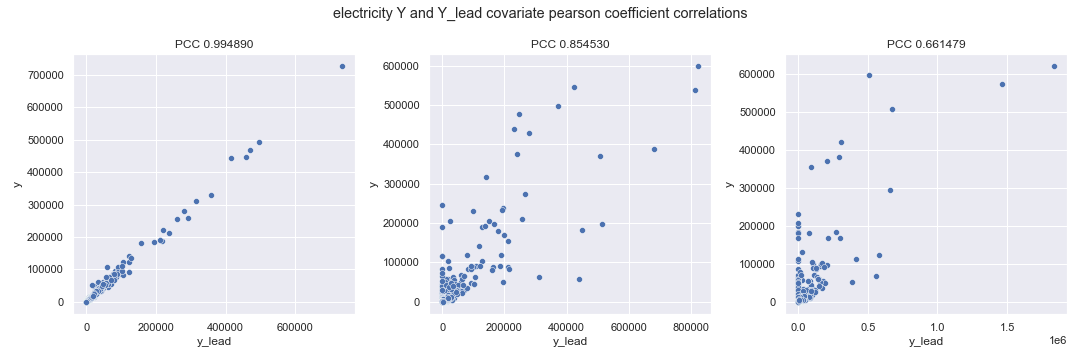
\includegraphics[width=0.8\textwidth]{figures/electricity-pcc.png}
\caption{Plots of various correlations between covariate and target variables on the Electricity dataset}
\label{fig:my_label}
\end{figure}

We then compute the cross correlation between the covariates and the target variables with the Pearson correlation coefficient ($\pearson$) 
and aim for each experiment to be run with a strong to perfect positive correlation in the range 0.5 to 1.0. This value is then directly 
comparable to autocorrelation of lagged variables.

%where the threshold for determining if a variable is autocorrelated 
%as opposed to being random white noise is calculated 
%as $\frac{2}{\sqrt{\timeserieslength}}$ \cite{hyndman2021forecasting} where $\timeserieslength$ is the length of the timeseries. For the \texttt{Hospital}
%dataset containing the shortest series this is $\approx0.21$, in otherwords each experiment is run in the presence of informative covariates. 


\subsection{Model architectures}
To better understand how covariates affect our results and attribute their impact more accurately, 
we employed two straightforward LSTM~\cite{HochSchm97} based architectures. Unlike the deep learning models benchmarked 
by Monash \cite{DBLP:conf/nips/GodahewaBWHM21} which used the GluonTS \cite{gluonts_arxiv} framework 
for training we did not add covariates such as lag variables and static time-series identifiers. 

Of these models: base-lstm is used as a baseline and is benchmarked against the Monash repository results using the same context length
and forecast horizons; while the seg-lstm model is intended to be more capable of forecasting over longer horizons using longer context lengths.


\subsubsection{Baseline model (base-lstm)}
Baseline is a vanilla LSTM~\cite{HochSchm97} with a scaling strategy inspired by DeepAR\cite{salinas2019deepar}.
The input data is scaled using mean absolute scaling within each mini-batch. An additional time dependent feature $\log(scale)$ is concatenated with the input vector. The scaled values are fed into a $2$ layer 
LSTM with each layer comprising of $40$ neurons. The output of the LSTM is then fed into a single fully connected layer 
with $40$ neurons with ReLU activations. Finally, an output layer generates a vector $\mathbf{z_t}$ 
containing the predicted target variable $\hat{y_t}$ and predicted covariates.  An inverse scaling operation finally transforms 
the predictions back into the original scale.

\subsubsection{Segment model (seg-lstm)}
The seg-lstm model addresses the limitation of the baseline model in forecasting over longer time horizons. 
Unlike GluonTS models, which incorporate lag variables, our approach aims to maximize historical data without relying on extra features.

To achieve this, we propose an LSTM with a simple modification to handle input data. We reshape each window of $T$ values 
into a vector of dimension $\frac{T}{d} \times d$, where $d$ represents the segment length, typically set to the seasonality
 of the data (e.g., 24 for hourly readings).

The model architecture is similar to the base-lstm, comprising a straightforward LSTM with 2 layers followed by fully connected 
layers with ReLU activations. We use mean absolute scaling but omit the additional time-dependent feature $\log(\text{scale})$.

During training, we compute the loss by comparing the last timestep of each segment output to the corresponding timestep in the 
target vector shifted one step into the future. The network is trained to predict one timestep ahead from each segment, with hidden 
state representations derived from segments separated by a time period $d$.

During inference, we predict the next timestep vector, append it to the previous timestep segment, and drop the oldest vector $z$. 
This forms an autoregressive loop, predicting successive segments of adjacent timesteps rather than spanning a fixed time period $d$.


\subsection{Evaluation Metrics}
We evaluate the performance of each model using MAE, RMSE, and sMAPE, computed on the raw (i.e., unscaled) 
values of the dataset. This approach ensures direct comparability with results from 
the Monash archive\cite{DBLP:conf/nips/GodahewaBWHM21}, enabling comprehensive assessment and comparison.

\begin{equation*}
\begin{aligned}
\text{MAE}(\hat{Y}, Y) &= \frac{ \sum_{\ts=1}^{\horizon}|\hat{Y}\ts - Y\ts|}{\horizon} &
\quad
\text{RMSE}(\hat{Y}, Y) &= \sqrt{\frac{\sum_{\ts=1}^{\horizon}(\hat{Y}_\ts - Y_\ts)^2}{\horizon}} \\
\text{sMAPE}(\hat{Y}, Y) &= \frac{100\%}{\horizon}\sum_{\ts=1}^{\horizon}\frac{|\hat{Y}_\ts - Y_\ts|}{(|\hat{Y}_\ts| + |Y_\ts|)/2}
\end{aligned}
\end{equation*}

\section{Experimental Setup}
We now describe in details of the experiments including how the data was processed, the 
model training and evaluation.

\subsection{Data Processing}
To facilitate model training, we generate time windows of data, each of which is equal in 
size to the sum of the context length ($\contextlength$) and the forecast horizon ($\horizon$). During each training epoch, 
complete and overlapping windows are extracted from each time series. 

% The number of available windows or samples for each dataset with $\datasettscount$ timeseries each containing $\timeserieslength$ 
% historical values is given by:

% \begin{equation}
% \sum_{k=1}^{\datasettscount} \timeserieslength - \contextlength - \horizon
% \end{equation}


%\subsection{Data Split}
The dataset is partitioned into training, validation, and test sets, following a chronological order. 
The validation set excludes values within the last forecast horizon, while the training set excludes 
values from the last two forecast horizons. Evaluation for both validation and testing is conducted 
on the last complete forecast horizon period of each time series. This approach maximizes the 
utilization of training data while preventing data leakage between the three sets.

%\subsection{Scaling}
We employ a variation of mean absolute scaling to standardize the data within in each mini-batch, 
accounting for divisions by zero. 
Covariates are scaled using the same scaling values to ensure consistency across features.

%\begin{equation}
%\text{scale}(\mathbf{y}, \mathbf{m} ) = 
%\text{max}(\frac{{\sum_{i} |\text{y}_{i} \cdot \text{m}_{i}|}}{{\sum_{i} \text{m}_{i}}},  1)
%\end{equation}
\begin{equation}
\text{scale}(\mathbf{y}) = 
\text{max}({{\sum_{i} |\text{y}_{i}|}},  1)
\end{equation}
  


%Where $\mathbf{m} = (m_1, m_2, \ldots, m_n)$ are the individual elements of the mask vector. Each  $m_i$
%can take on either 0 or 1 to indicate the presence or absence of masked values. $\mathbf{y}$ is the vector
%of the target variable from previous timesteps representing context which will condition the neural network. 


\subsection{Training}
We utilized teacher forcing which trains the network to predict a single
timestep ahead and calculated the loss for the entire sequence (ie the context length and the forecast horizon).
The network was trained as a regression task with a Smooth F1 Loss objective.
%
%We treat the training as a regression task and 
%considered using Mean Squared Error (MSE) as an objective function but selected the Smooth F1 Loss objective, 
%which we found to exhibit slightly better performance. 

\begin{equation}
\text{SmoothL1Loss}(\hat{y}, y) = 
\begin{cases} 
0.5(\hat{y} - y)^2 & \text{if } |\hat{y} - y| < 1 \\
|\hat{y} - y| - 0.5 & \text{otherwise}
\end{cases}
\end{equation}

A number of hyperparameters were set to match the default
GluonTS parameters \cite{gluonts_arxiv} including weight decay \cite{loshchilov2019decoupled} of $1e-8$; dropout 
\cite{hinton2012improving} of 0.1; and a learning rate of 0.001. We used OneCycle \cite{smith2018superconvergence} scheduling to increase and then 
anneal the learning rate over 100 epochs. The models were optimized using AdamW.

Performance was measured on the validation set at the end of each epoch by measuring the Smooth L1 loss using
free running (ie using the predicted outputs of one timestep as the input into the next). The model checkpoint
with the lowest validation loss was selected for testing. The hidden state of the the LSTM was initialised to $0$. 


% It's worth noting here that there are two possible approaches to generating autoregressive outputs from recurrent networks. One method
% is to condition the LSTM with the historical context values which produces a hidden state and output from which to generate
% successive predictions which is done by "unrolling" the LSTM and passing in the hidden state and output recursively until 
% the desired number of outputs are generated. In this arrangement the state initialised once prior to the historical context 
% being processed. 

% An alternative is to return only 1 timestep ahead at a time and require the calling process to construct 
% a new historical context (utilising the previous timestep prediction). If the historical context
% is kept at a constant size then the oldest value from the context is dropped between each successive output generation. In this scenario
% the hidden state is reinitialised between each generated timestep which might seem to be problematic. However this approach does offer
% the opportunity to recalculate the scale values at each timestep. 

% In practice we found that both approaches performed much the same and the experiments were run with the latter approach
% as training teacher forcing setup was more computationally efficient.

\subsection{Experimental Procedure}
Initially, we trained models for each dataset using the context length and forecast horizon values consistent with 
those used in the Monash repository which allowed us to compare the performance of our models 
against benchamrked results. Next, we trained and evaluated models under various scenarios involving 1, 2, and 3 
covariates. For each scenario:

\begin{itemize}
  \item We trained a univariate model without covariates to predict a forecast horizon equal to the number of covariates being 
  tested.
  \item For the number of covariates in the scenario a set of base-lstm models were trained with increased noise to vary the 
  level of cross correlation with the target variables.  This allows us to assess the impact of covariates on model performance under 
  different correlation levels. These models were trained to a context length and forecast horizon that equalled the benchmarked 
  results from Monash \cite{DBLP:conf/nips/GodahewaBWHM21}
 \item We then trained a seg-lstm models using the same procedure as in the prior step with the exception that we use a longer context 
 length which was set to 3x the forecast horizon on \texttt{Hospital}, \texttt{Tourism} and \texttt{Electricity} and 8x the forecast horizon on \texttt{Traffic}. 
\end{itemize}

\section{Results}
Table \ref{tab:benchmark} presents the mean error metrics for each dataset evaluated against the neural network architectures benchmarked 
by Godahewa et al \cite{DBLP:conf/nips/GodahewaBWHM21}. Among these architectures, FFNN and N-BEATS \cite{oreshkin2020nbeats} are fully-connected models, 
while DeepAR \cite{salinas2019deepar} is based on an LSTM network. WaveNet \cite{oord2016wavenet}, originally designed for 
audio synthesis, was adapted by Alexandrov et al \cite{gluonts_arxiv} for time-series tasks in GluonTS. Additionally, the Transformer 
architecture closely follows the implementation described in the original paper by Vaswani et al \cite{vaswani2023attention}.

Comparing the base-lstm model across datasets, it yielded comparable results on the \texttt{Hospital} and \texttt{Traffic} datasets, 
slightly inferior results on \texttt{Tourism}, and significantly poorer results on \texttt{Electricity} when measured by sMAPE. However, 
the performance marginally improved when evaluated using MAE and RMSE. Notably, the base-lstm model exhibited relatively better performance on datasets with shorter forecast horizons.

The seg-lstm model emerged as the top performer on Electricity with RMSE and second with MAE and sMAPE, whilst on \texttt{Tourism} it ranked second  
with MAE and RMSE , both of which have longer forecast horizons. Overall, both of our models demonstrated comparable performance to the benchmarks on the shorter forecast 
horizons of \texttt{Hospital} and \texttt{Traffic}, while the seg-lstm model also displayed competitive performance on \texttt{Tourism} 
and \texttt{Electricity}.



\begin{table}[tbp]
  \caption{Benchmark error for each dataset. Reference values taken from \cite{DBLP:conf/nips/GodahewaBWHM21}. Forecast horizons are given in the brackets }
  \centering
  \begin{threeparttable}
  \begin{small}
  \renewcommand{\multirowsetup}{\centering}
  \setlength{\tabcolsep}{2.6pt}
  \begin{tabular}{c|c|ccccccc}
    \toprule
    \multicolumn{2}{c}{Models} & \multicolumn{1}{c}{FFNN} &  \multicolumn{1}{c}{DeepAR} & \multicolumn{1}{c}{N-Beats}  & \multicolumn{1}{c}{Wavenet} & \multicolumn{1}{c}{Transformer} & \multicolumn{1}{c}{base-lstm} & \multicolumn{1}{c}{seg-lstm}  \\
    \toprule
    \multirow{3}{*}{\rotatebox{90}{Hosp}} 
    & sMAPE &  18.33         & \textbf{17.45}   & 17.77            & 17.55            & 20.08                              & 17.52                           & 18.05                           \\
    & MAE   & 22.86         & 18.25   & 20.18            & 19.35            & 36.19                              & \textbf{18.03}                            & 19.95                     \\
    & RMSE &  27.77         & \textbf{22.01}   & 24.18            & 23.38            & 40.48                              & 22.03                            & 24.19                     \\
    \midrule
    \multirow{3}{*}{\rotatebox{90}{Tourism}}
    & sMAPE  & 20.11         & \textbf{18.35}   & 20.42            & 18.92            & 19.75                              & 21.50                           & 19.85                           \\
    & MAE   & 2022.21       & \textbf{1871.69} & 2003.02          & 2095.13          & 2146.98                            & 2336.42                        & 1956.07                         \\
    & RMSE  & 2584.10       & \textbf{2359.87} & 2596.21          & 2694.22          & 2660.06                            & 2964.96                        & 2413.64                         \\
    \midrule
    \multirow{3}{*}{\rotatebox{90}{Traffic}} 
    & sMAPE & 12.73         & 13.22            & 1\textbf{2.40}   & 13.30            & 15.28                            & 12.77                           & 12.97                           \\
                      & MAE   & 1.15          & 1.18             & \textbf{1.11}    & 1.20             & 1.42                               & 1.15                            & 1.17                           \\
                      & RMSE  & 1.55          & 1.51             & \textbf{1.44}    & 1.61             & 1.94                               &  1.56                           & 1.58                           \\
    \midrule
    \multirow{3}{*}{\rotatebox{90}{Elec}}  
    & sMAPE & 23.06         & \textbf{20.96}   & 23.39            & -                & 24.18                              & 34.12                           & 21.20                           \\
                      & MAE   & 354.39        & 329.75           & 350.37           & \textbf{286.56}  & 398.80                             & 525.50                          & 287.95                         \\
                      & RMSE  & 519.06        & 477.99        & 510.91           & 489.91           & 514.68                             & 675.03                          & \textbf{469.07}               \\
    \bottomrule
  \end{tabular}
\end{small}
\end{threeparttable}
\vspace{-15pt}
\label{tab:benchmark}
\end{table}

\subsection{Covariates}
Moving on to the experiments with covariates we note some common characteristics across all 4 datasets. 

The relative differences in performance between univariate and covariates cases at the full forecast horizons is somewhat specific to the dataset. Table \ref{tab:covariate_results} shows the results at 
full forecast horizons. Of the datasets tested \texttt{Traffic} exhibits the best performance advantage sMAPE of 9.5\% with covariate compared to 12.5\% as univariate. The underlying 
reason for this will be discussed later. In contrast covariate models on \texttt{Tourism} carry a penalty as performance is inferior at all correlations levels. 

The shorter forecast horizon datasets of \texttt{Hospital} and \texttt{Traffic} exhibit improved performance as the number of covariates increases. This effect is more 
pronounced as the $\pearson$ increases. The base-lstm sMAPE on \texttt{Traffic} improves from 8.14 with 1 covariate to 5.92 with 3 covariates.

\begin{table}[tbp]
  \caption{sMAPE results for covariates $k \in \{1, 2, 3\}$ with different $\pearson$ values. We set the $\horizon$ to match the Monash benchmark values }
  \centering
  \begin{threeparttable}
  \begin{small}
  \renewcommand{\multirowsetup}{\centering}
  \setlength{\tabcolsep}{2.6pt}
  \begin{tabular}{c|c|cccccccccccccc}
    \toprule
    \multicolumn{2}{c}{Models} & \multicolumn{3}{c}{\textbf{base-lstm}} & \multicolumn{3}{c}{\textbf{seg-lstm}} \\
    \cmidrule(lr){3-5} \cmidrule(lr){6-8}
    \multicolumn{2}{c}{$\pearson$} & 1 & 0.9 & 0.5 & 1 & 0.9 & 0.5 \\
    \toprule
    \multirow{4}{*}{\textbf{Hospital}} & 0 & 17.52 $\pm$ 0.041 & 17.52 $\pm$ 0.041 & 17.52 $\pm$ 0.041 & 18.05 $\pm$ 0.135 & 18.05 $\pm$ 0.135 & 18.05 $\pm$ 0.135 \\
    & 1 & 15.98 & 17.34 & 17.43 & 16.47 & 18.06 & 18.39 \\
    & 2 & 14.68 & 17.32 & 17.59 & 14.87 & 18.09 & 18.12 \\
    & 3 & 13.53 & 17.07 & 17.33 & 13.96 & 18.24 & 18.62 \\
    \midrule
    \multirow{4}{*}{\textbf{Tourism}} & 0 & 21.50 $\pm$ 0.531 & 21.50 $\pm$ 0.531 & 21.50 $\pm$ 0.531 & 19.85 $\pm$ 0.62 & 19.85 $\pm$ 0.62 & 19.85 $\pm$ 0.62 \\
    & 1 & 19.97 & 23.76 & 25.96 & 18.81 & 23.43 & 21.13 \\
    & 2 & 20.54 & 23.76 & 26.65 & 17.76 & 20.23 & 22.86 \\
    & 3 & 20.93 & 24.19 & 29.57 & 19.80 & 21.76 & 24.07 \\
    \midrule
    \multirow{4}{*}{\textbf{Traffic}} & 0 & 12.77 $\pm$ 0.065 & 12.77 $\pm$ 0.065 & 12.77 $\pm$ 0.065 & 12.97 $\pm$ 0.108 & 12.97 $\pm$ 0.108 & 12.97 $\pm$ 0.108 \\
    & 1 & 8.14 & 9.24 & 9.49 & 8.50 & 9.42 & 9.45 \\
    & 2 & 6.85 & 8.58 & 9.25 & 7.15 & 8.82 & 9.23 \\
    & 3 & 5.92 & 8.27 & 9.15 & 6.57 & 8.86 & 9.56 \\
    \midrule
    \multirow{4}{*}{\textbf{Electricity}} & 0 & 34.12 $\pm$ 2.38 & 34.12 $\pm$ 2.38 & 34.12 $\pm$ 2.38 & 21.20 $\pm$ 0.232 & 21.20 $\pm$ 0.232 & 21.20 $\pm$ 0.232 \\
    & 1 & 34.59 & 30.88 & 36.62 & 20.66 & 22.08 & 21.99 \\
    & 2 & 35.27 & 31.59 & 32.01 & 20.52 & 21.21 & 21.50 \\
    & 3 & 44.09 & 33.39 & 31.35 & 20.75 & 22.52 & 22.87 \\
    \bottomrule
  \end{tabular}
  \end{small}
  \end{threeparttable}
  \label{tab:covariate_results}
  \vspace{-15pt}
\end{table}

Figure \ref{fig:lstm_smape_vs_pearson} shows how the error degrades as a function of $\pearson$ on each of the datasets where the 
forecast horizon is 3.  At short forecast horizons where the $\horizon <= max(k)$ 
and k is leading time steps, the performance is an almost perfect prediction when the  cross correlation is $\pearson$ = 1.0 (ie perfect correlations) and progressively worsens with additional noise.


\begin{figure}[ht]
\centering
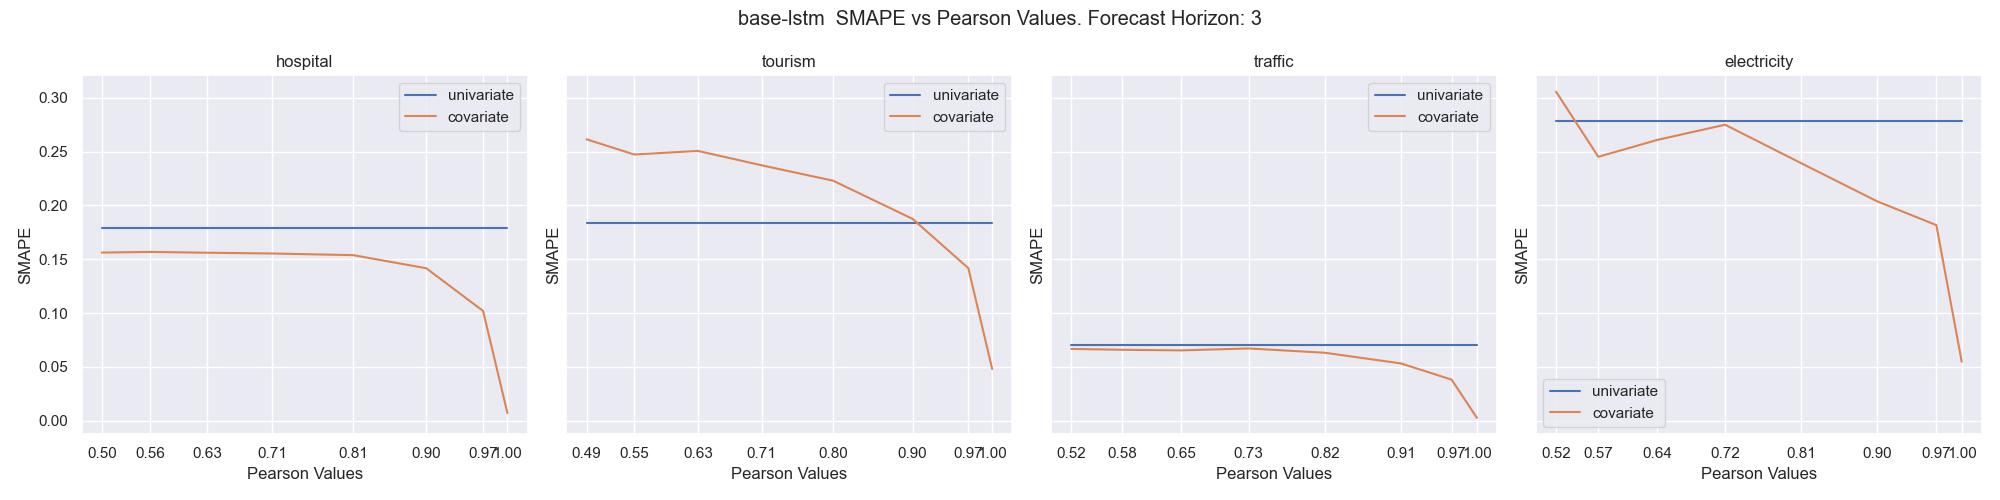
\includegraphics[width=0.9\textwidth]{figures/base-lstm_smape_vs_pearson.png}
\caption{base-lstm smape as a function of PCC for 3 covariates}
\label{fig:lstm_smape_vs_pearson}
\end{figure}


The performance advantage over a univariate case diminishes as the forecast horizon extends and in most cases for a $\pearson$ value of 0.9 and below is negated 
or even worse for forecast horizons that exceed 4-5 timsteps. Figure \ref{fig:hospital_smape} shows the sMAPE as a function of forecast horizon and shows the errors 
converge at from forecast horizon at 4 timesteps for $\pearson$ of 0.81 and lower.

\begin{figure}[ht]
\centering
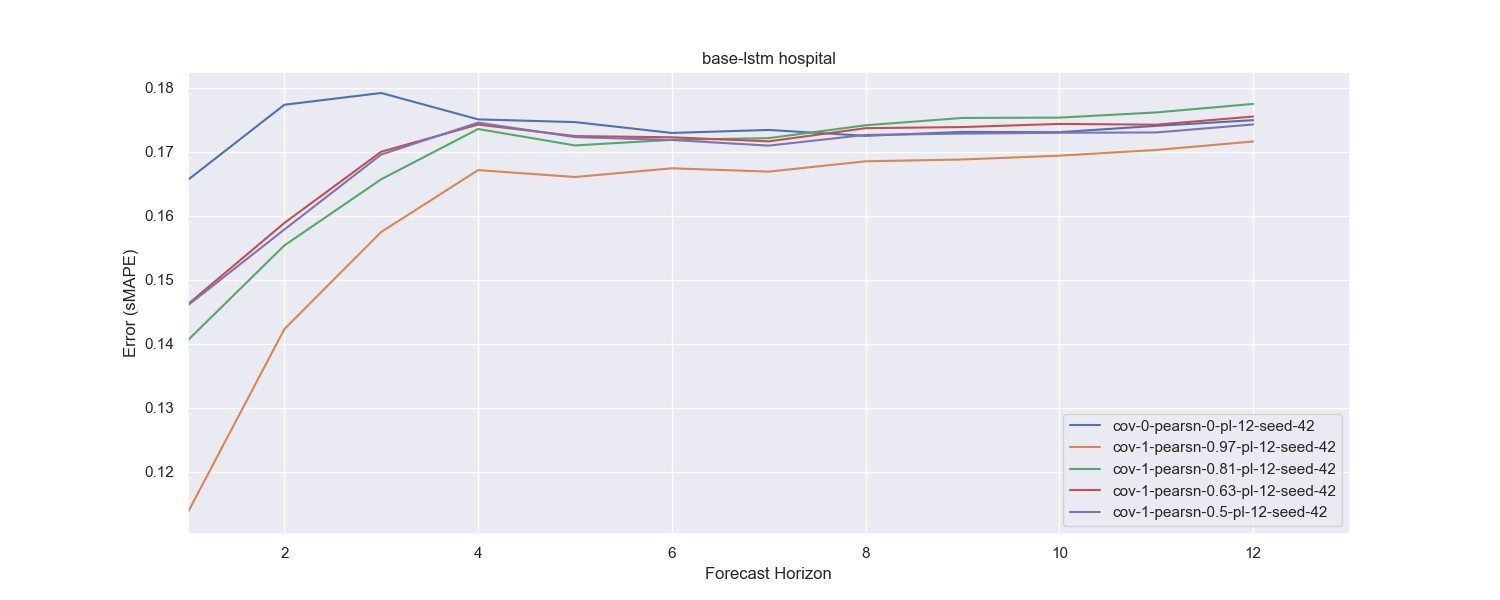
\includegraphics[width=0.9\textwidth]{figures/base-lstm-hospital-sMAPE.png}
\caption{base-lstm Hospital smape as a function of forecast horizon for 1 covariate}
\label{fig:hospital_smape}
\end{figure}

Looking at the differences between base-lstm and seg-lstm. We see that both models share common characteristics. The relative differences between univariate 
and covariates share similar patterns for each of the datasets. The longer forecast horizons of Tourism and Electricity show an improvement in absolute performance 
but there relative differences are much the same. Figure \ref{fig:tourism_base_vs_seg}


\begin{figure}[ht]
  \centering
  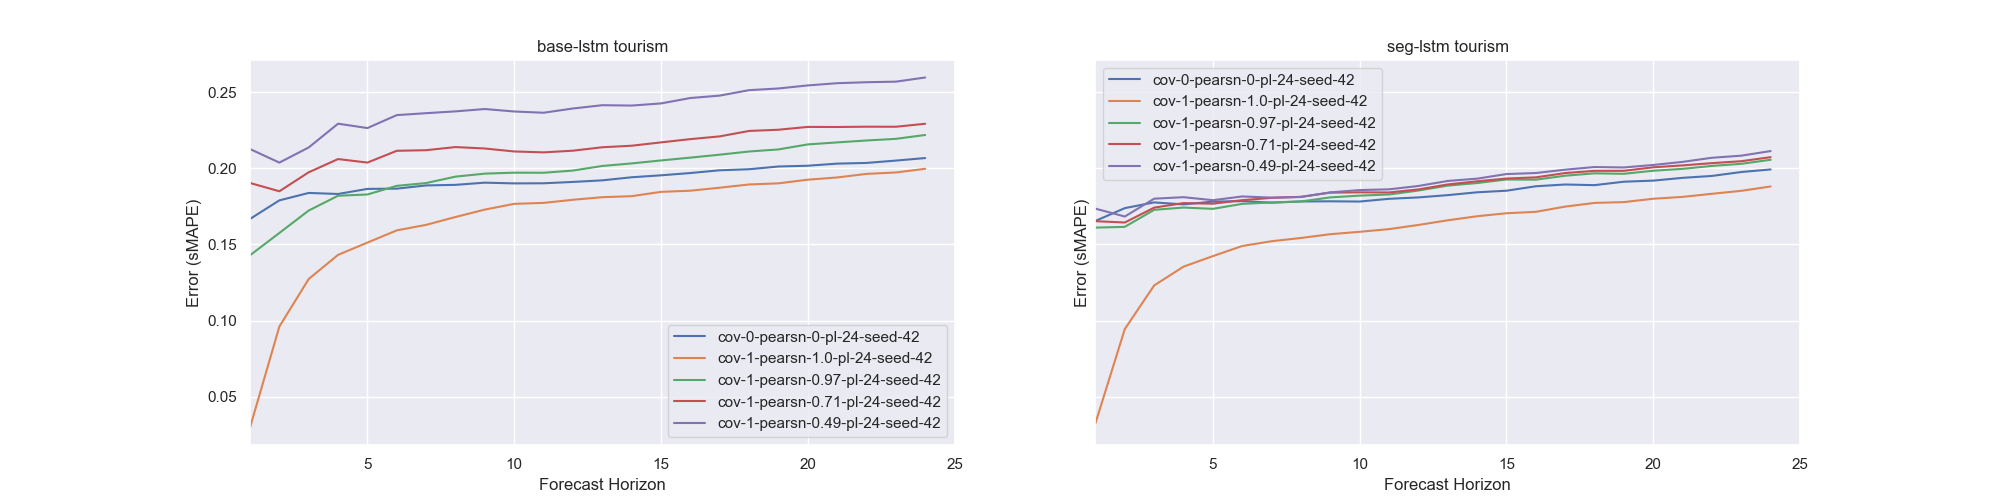
\includegraphics[width=1.\textwidth]{figures/tourism_base-lstm_vs_seg-lstm.png}
  \caption{Tourism smape for 1 covariate for base-lstm and seg-lstm}
  \label{fig:tourism_base_vs_seg}
  \end{figure}
  


Turning to using multiple covariates. Fig \ref{fig:lstm_traffic_univariate_vs_covariate} show sMAPE across full forecast horizons for 1, 2 and 3 covariates. Note that the error lags univariate with the timesteps 
that lag the univariate case being equal to the maximum leading covariate timestep. ( ie the error lag is 1 timestep for 1 covariate, 2 timesteps for 2 covariates and so on). A similar pattern 
is observed on the \texttt{Electricity} and to a lesser degree on the \texttt{Tourism} dataset. 


\begin{figure}[ht]
  \centering
  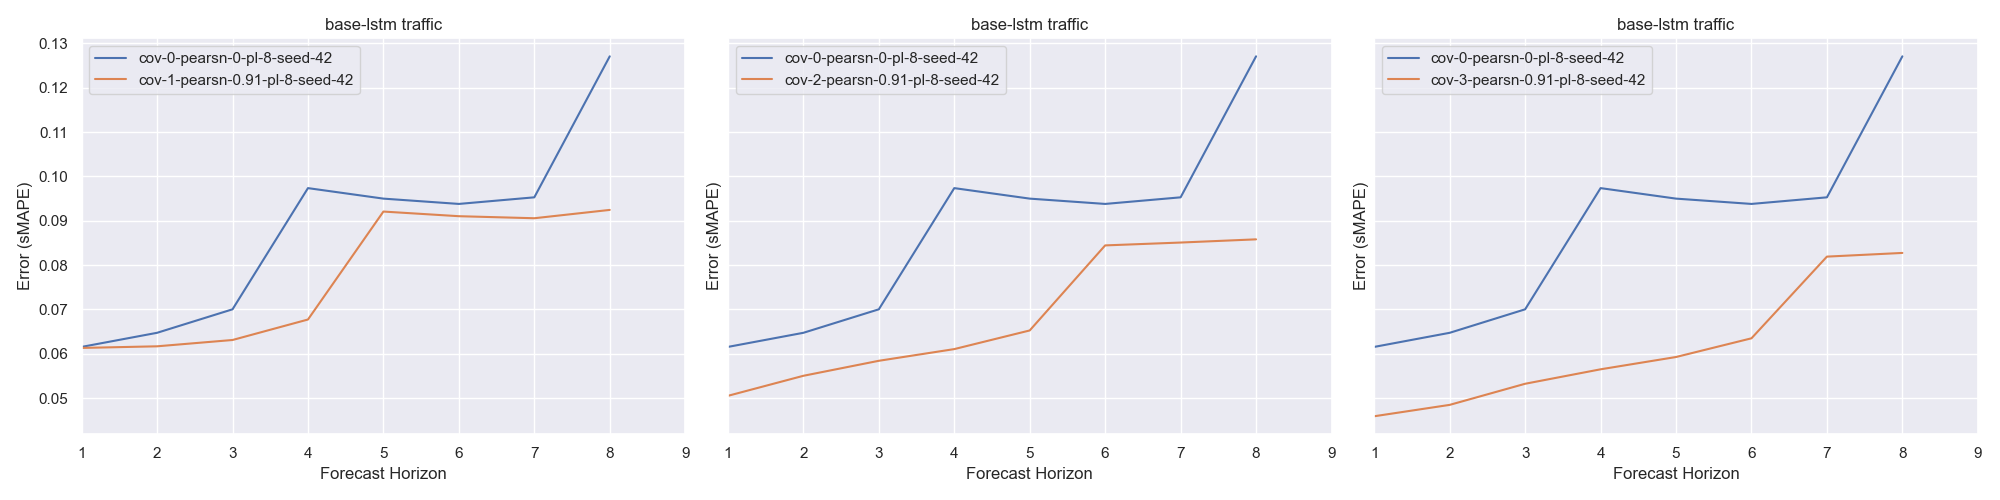
\includegraphics[width=1.\textwidth]{figures/base-lstm_traffic_univariate_vs_covariate.png}
  \caption{Traffic smape comparing univariate to 1, 2 and 3 covariates for base-lstm at a $\pearson$ = 0.9}
  \label{fig:lstm_traffic_univariate_vs_covariate}
  \end{figure}
  


We argue that this delay of error pattern of errors across forecast horizons demonstrates 
that the network is effectively utilising all the covariates available. The question then is to determine whether the network is just utilising the covariates at the current timestep 
or whether the it can learn from temporal and feature dimension simultaneously. We can test the hypothesis that the network does learn using both temporal 
and feature dimensions by repeating the experiment with a simple modification. We have a feature vector containing covariates $x_1, x_2, x_3$ which provide information 
about the target values at timesteps $t_1, t_2, t_3$ respectively. If the covariate $x_2$ is removed then the only way the network can obtain information about the 
target value at $t_2$ is to use the $x+3$ covariate from the previous timestep. We argue that if in this experiment we observe a similar pattern as was observed with 
using covariates $x_1, x_2, x_3$ then the network must be learning temporal and feature dimensions simultaneously. Conversely, if the error follows a different pattern
possibly looking similar to using a single covariate $x_1$ then we can conclude that the network is learning the covariates from only the current timestep. 

Fig TODO shows plots of this test on the \texttt{Traffic} dataset with a $\pearson$ where it is clear that the error does emulate the error of using 
3 covariates and therefore we argue that the lstm does indeed learn covariates across both feature and temporal dimensions simultaneously.



We conclude that:
\begin{itemize}
\item the lstm is able to model both temporal and feature dynamics at short forecast horizons in the presence short lead timestep covariates.
\item The magnitude of the performance gain is related to the strength of the correlation between the covariate and the target variables and that this relationship 
is non-linear with performance degrading most rapidly for $\pearson$ levels between 1.0 and 0.9. 
\item Any advantage from covariates where $\pearson$ is below 0.9 rapidly diminishes as forecast horizons extend beyond 4-5 timesteps and quite often error will continue to decline more rapidly than 
the univariate case (ie the presence of covariates becomes a hinderence to performance. )
\item The number of timesteps covered by multiple covariates can be combined to provide a short term performance advantage. 
\item The magnitude of the performance advantage from using covariates is related to the model's underlying ability to forecast accurately. In other words models that are 
inherently produce better performance in a univariate setting will produce better results in a covariate setting. 
\item Increasing the number of covariates can enhance performance on short forecast horizons with the magnitude of the performance being related to the $\pearson$
\end{itemize}

\section{Discussion}

Given the aim of this study to explore the effect of covariates on LSTM networks, it's evident that predicting covariates 
jointly with target variables can under certain conditions result in a performance improvement, however frequently is can in fact hinder performance. 
Furthermore, the performance benefit quickly diminishes as the correlation between covariates and target variables 
decreases.  While acknowledging the artificial nature of such high correlations, used in this study
it nonetheless underscores the potential for covariates to assist neural networks in making more accurate predictions, 
albeit under somewhat artificial conditions. Future studies could evaluate the use of covariates with more representative 
real-world data, such as the work by Wang et al. (2006) \cite{wang2006} on predicting UK spirit consumption using wealth as a covariate. 
Additionally, further exploration with artificial datasets could investigate the effects of other characteristics like 
non-stationarity or negative correlations.




Finally, it may be possible that LSTM's may struggle to learn the relationships between covariates and target variables 
across both the temporal and feature dimensions while simultaneously generating a vector output in an autoregressive 
manner. This raises questions about the potential benefits of incorporating mechanisms like attention, either as an 
extension to the LSTM or through the adoption of a transformer network. Alternatively, it prompts consideration of whether 
supplying the network with information about the number of timesteps each leading indicator will affect the target variable 
could simplify the learning task.



%When testing covariates on a 1, 2, 3 
%step forecast horizon with perfectly correlated covariates unsurprisingly we see the error drop to produce an almost perfect prediction. 
%\texttt{Hospital} sMAPE is 0.6\% - 0.7\%. \texttt{Tourism} is 3.8\% - 4.8\%, \texttt{Traffic} is 0.3\%. From this we concluded the model was able to utilise the leading covariates effectively.

%The second common characteristic is that the performance degrades as more noise is added to the covariates and typically the rate of decline is at it's greatest
%between a ($\pearson$) of 1 (ie perfect correlation) and 0.9. 



  


%Figure \ref{fig:hospital_smape} are plots of sMAPE measured with various covariates and forecast horizons. With the forecast horizons set the to match the number of covariates the models
%outperfom the baseline model consistently across all values of $\pearson$. At a $\pearson$ of 0.5 with 1 covariate the sMAPE is 1.8\% points better 
%than the baseline of 16.5\%. This pattern is repeated for 2 and 3 covariates. 

%With the full forecast horizon of 12 timesteps (1 year) and a context length of 15 the benefit from using covariates is essentially negated with 
%a $\pearson$ of 0.9 and below.

%Figures \ref{fig:base_lstm_hospital_mae} and \ref{fig:base_lstm_hospital_rmse} show the relative differences between baseline and covariate presence measured with MAE and RMSE are worse than sMAPE, and in the case of the full 
%forecast horizon are worse than baseline. 

%The same pattern is observed with seg-lstm model.


%\subsection{Tourism}
%\begin{figure}[ht]
%\centering
%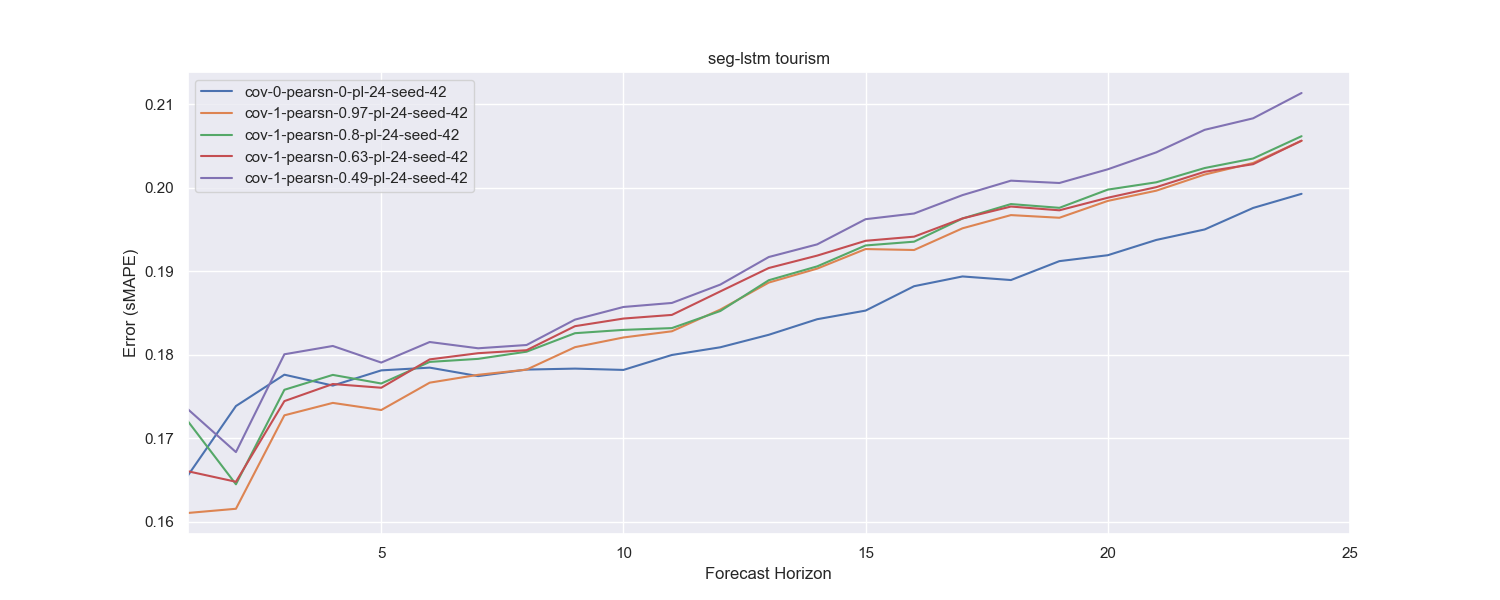
\includegraphics[width=0.9\textwidth]{figures/seg-lstm-tourism-sMAPE.png}
%\caption{seg-lstm Tourism smape as a function of forecast horizon correlation for 1 covariate}
%\label{fig:tourism_smape}
%\end{figure}
  
%The tourism dataset has been benchmarked with a forecast horizon of 24 (2 years) and a context length of 15. With this being a monthly dataset we expect 
%the seasonal length to be 12 months and so in some respects this is similar to the Hospital dataset in that the context length exceeds the season, but is 
%a more challenging task as the forecast horizon is twice as long. 

%In this case the results show inferior performance using covariates generally and the only occaisions where it performs better is then the $\pearson$ 
%is above 0.95 on short forecast horizons. In the extreme case the sMAPE is ~ 10\% points worse using covarariates. 


%\subsection{Traffic}
%\begin{figure}[ht]
%\centering
%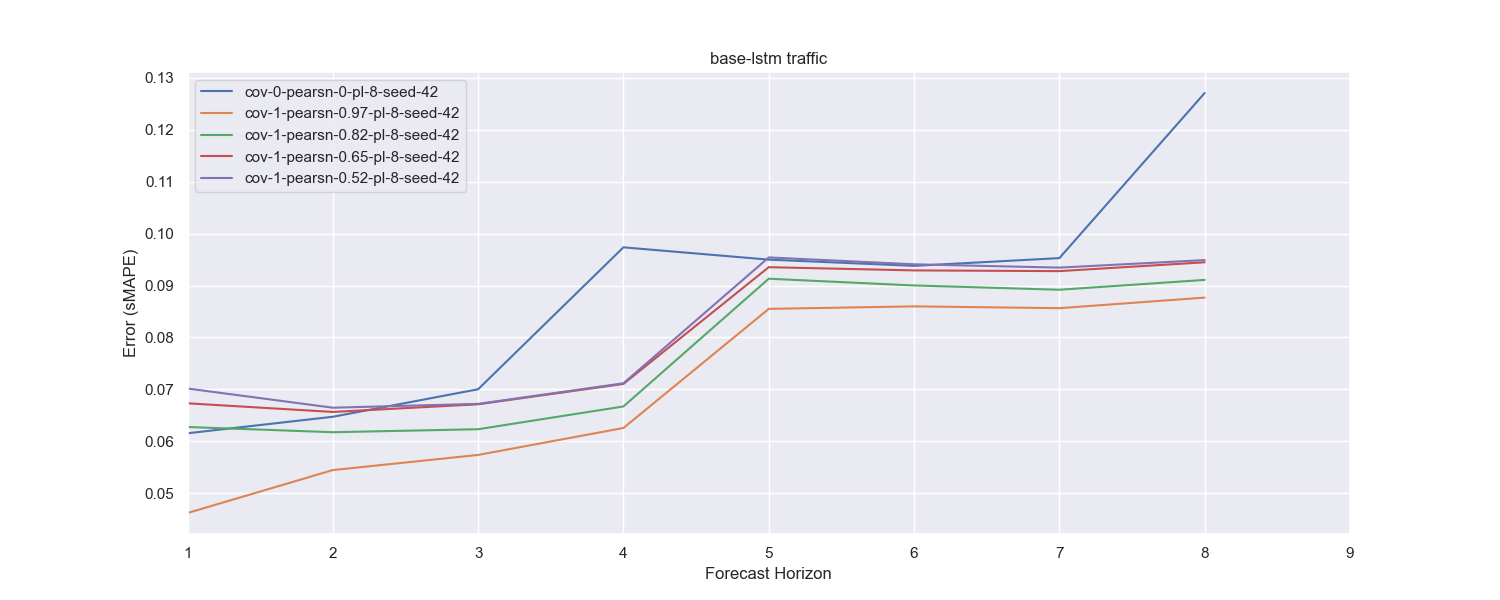
\includegraphics[width=0.9\textwidth]{figures/base-lstm-traffic-sMAPE.png}
%\caption{base-lstm Traffic smape as a function of forecast horizon correlation for 1 covariate}
%\label{fig:traffic_smape}
%\end{figure}

%The \texttt{traffic} dataset is weekly meaning that the seasonal length is 52 (ie 1 year). The context length used is 65 weeks (1 year 3 months) and the forecast 
%horizon is 8 weeks giving the highest ratio of context length to forecast horizon across all the datasets that we tested.

%When we examine the results with the shorter forecast horizon the relative difference in sMAPE between univariate and covariate 
%models becomes almost insignificant from a $\pearson$ 0.8 and below. Somewhat counterintuively the full forecast horizon has a 
%significantly lower sMAPE for covariate models with a 4-4.5\% point difference which was the largest difference of all the datasets evaluated. 

%However note that the univariate base\_smape error for the shorter forecast horizon is significantly lower than 
%for the full forecast horizon. In other words the univariate performance degrades more rapidly as the forecast horizon increases than the models 
%with covariates.

%\subsection{Electricity}
%\begin{figure}[ht]
%centering
%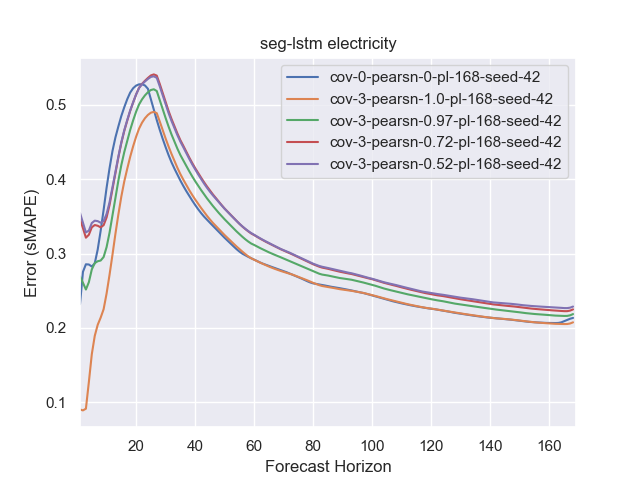
\includegraphics[width=0.9\textwidth]{figures/seg-lstm-electricity-sMAPE.png}
%\caption{seg-lstm Electricity smape as a function of forecast horizon for 1 covariate}
%\label{fig:electricity_smape}
%\end{figure}

%\texttt{Electricity} has by far the longest forecast horizon of 168 timesteps, but a context length of 30 meaning in other words the network is provided with 
%1 day and 6 hours of historical observations and is expected to predict the next 7 days of hourly values. It is the dataset that the base-lstm performed 
%worse on, however the sMAPE of 34.12\% is lower than the 40.47\% reported with TBATS by Monash \cite{DBLP:conf/nips/GodahewaBWHM21}.

%The shorter forecast horizons generally show an improvement over the univariate models although low ${\pearson}$ with 1 covariate are worse.  
%with the number of covariates and forecast horizon. In a similar pattern to the full forecast horizon with \texttt{Traffic} note that the 
%univariate sMAPE degrades significantly between 1 and 3 timestep forecast horizons.

%Forecasting the full 168 timesteps the relative differences between univariate and covariate models is worse with covariate models 
%on averge by circa 5\% points.

%\section{Discussion}
%The influence of covariates on model performance varies across different datasets, which is intriguing. 
%Among the four datasets examined, \texttt{Electricity} and \texttt{Hospital} display a similar pattern in their response 
%to covariates. In these cases, covariates exhibit minimal impact on performance over the entire forecast horizon. 
%However, they enhance performance notably for short forecast horizons, particularly evident when considering three 
%timesteps where baseline performance deteriorates while covariate performance remains stable.

%In contrast, the \texttt{Traffic} dataset shows a reversal in the relative performance between long and short horizons, 
%with performance improvement observed with longer forecast horizons. Nonetheless, it's important to note that the 
%variance of the error with covariates is considerably smaller than without, raising questions about whether covariates 
%contribute to greater stability across different forecast horizons and if this can be leveraged in scenarios where 
%model performance would otherwise degrade significantly.

%The \texttt{Tourism} dataset presents scenarios where the use of covariates significantly hinder performance, necessitating 
%further investigation into the underlying causes.

%Given the aim of this study to explore the effect of covariates on LSTM networks, it's evident that predicting covariates 
%jointly with target variables can under certain conditions result in a performance improvement, however frequently is can in fact hinder performance. 
%Furthermore, the performance benefit quickly diminishes as the correlation between covariates and target variables 
%decreases.  While acknowledging the artificial nature of such high correlations, used in this study
%it nonetheless underscores the potential for covariates to assist neural networks in making more accurate predictions, 
%albeit under somewhat artificial conditions. Future studies could evaluate the use of covariates with more representative 
%real-world data, such as the work by Wang et al. (2006) \cite{wang2006} on predicting UK spirit consumption using wealth as a covariate. 
%Additionally, further exploration with artificial datasets could investigate the effects of other characteristics like 
%non-stationarity or negative correlations.

%Finally, it is posited that an LSTM may struggle to learn the relationships between covariates and target variables 
%across both the temporal and feature dimensions while simultaneously generating a vector output in an autoregressive 
%manner. This raises questions about the potential benefits of incorporating mechanisms like attention, either as an 
%extension to the LSTM or through the adoption of a transformer network. Alternatively, it prompts consideration of whether 
%supplying the network with information about the number of timesteps each leading indicator will affect the target variable 
%could simplify the learning task.


\bibliographystyle{plain}
\bibliography{rnn-covariates}  % replace 'your_bib_file_name' with the name of your .bib file, without the extension


%%%%%%%%%%%%%%%%%%%%%%%%%%%%%%%%%%%%%%%%%%%%%%%%%%%%%%%%%%%%

\appendix

\section{Appendix / supplemental material}

\subsection{Hospital base-lstm plots}
\begin{figure}[htbp]
\centering
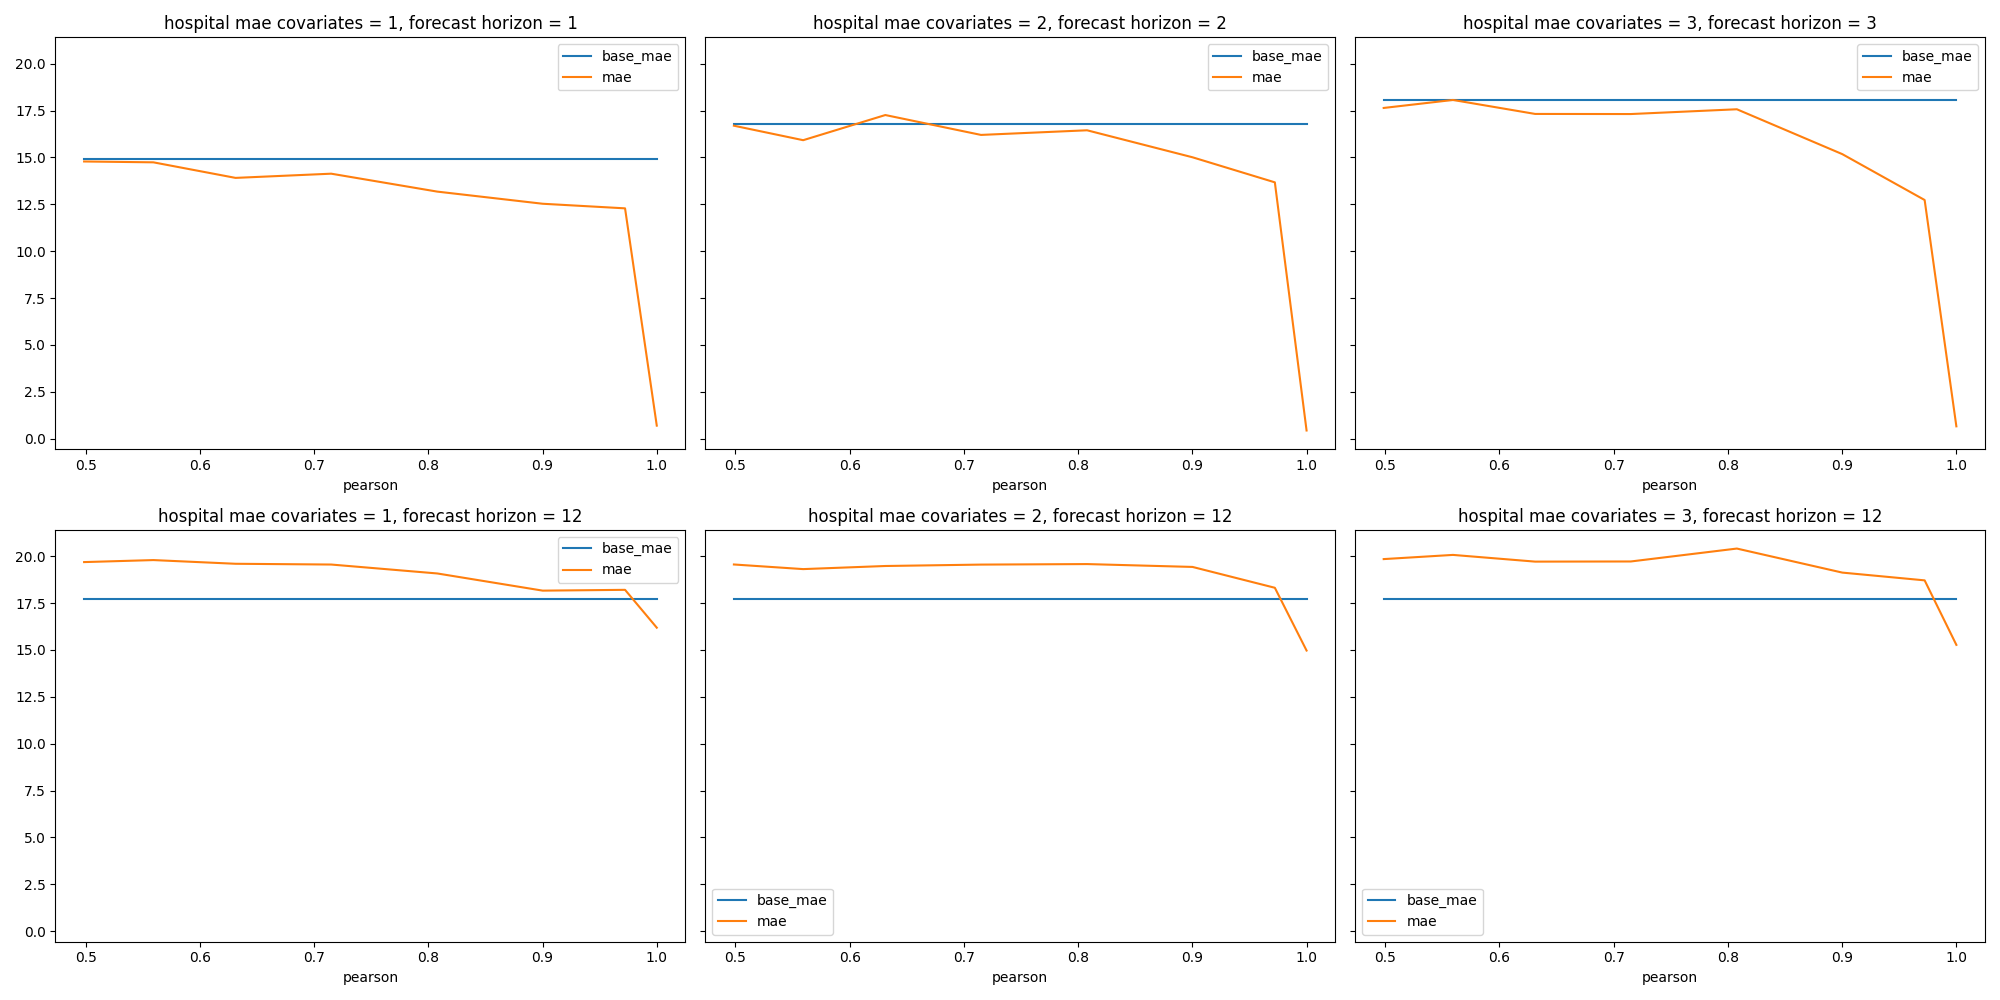
\includegraphics[width=0.9\textwidth]{figures/hospital-base-lstm-mae.png}
\caption{base-lstm Hospital mae as a function of correlation for 1, 2 and 3 covariates}
\label{fig:base_lstm_hospital_mae}
\end{figure}

\begin{figure}[ht]
\centering
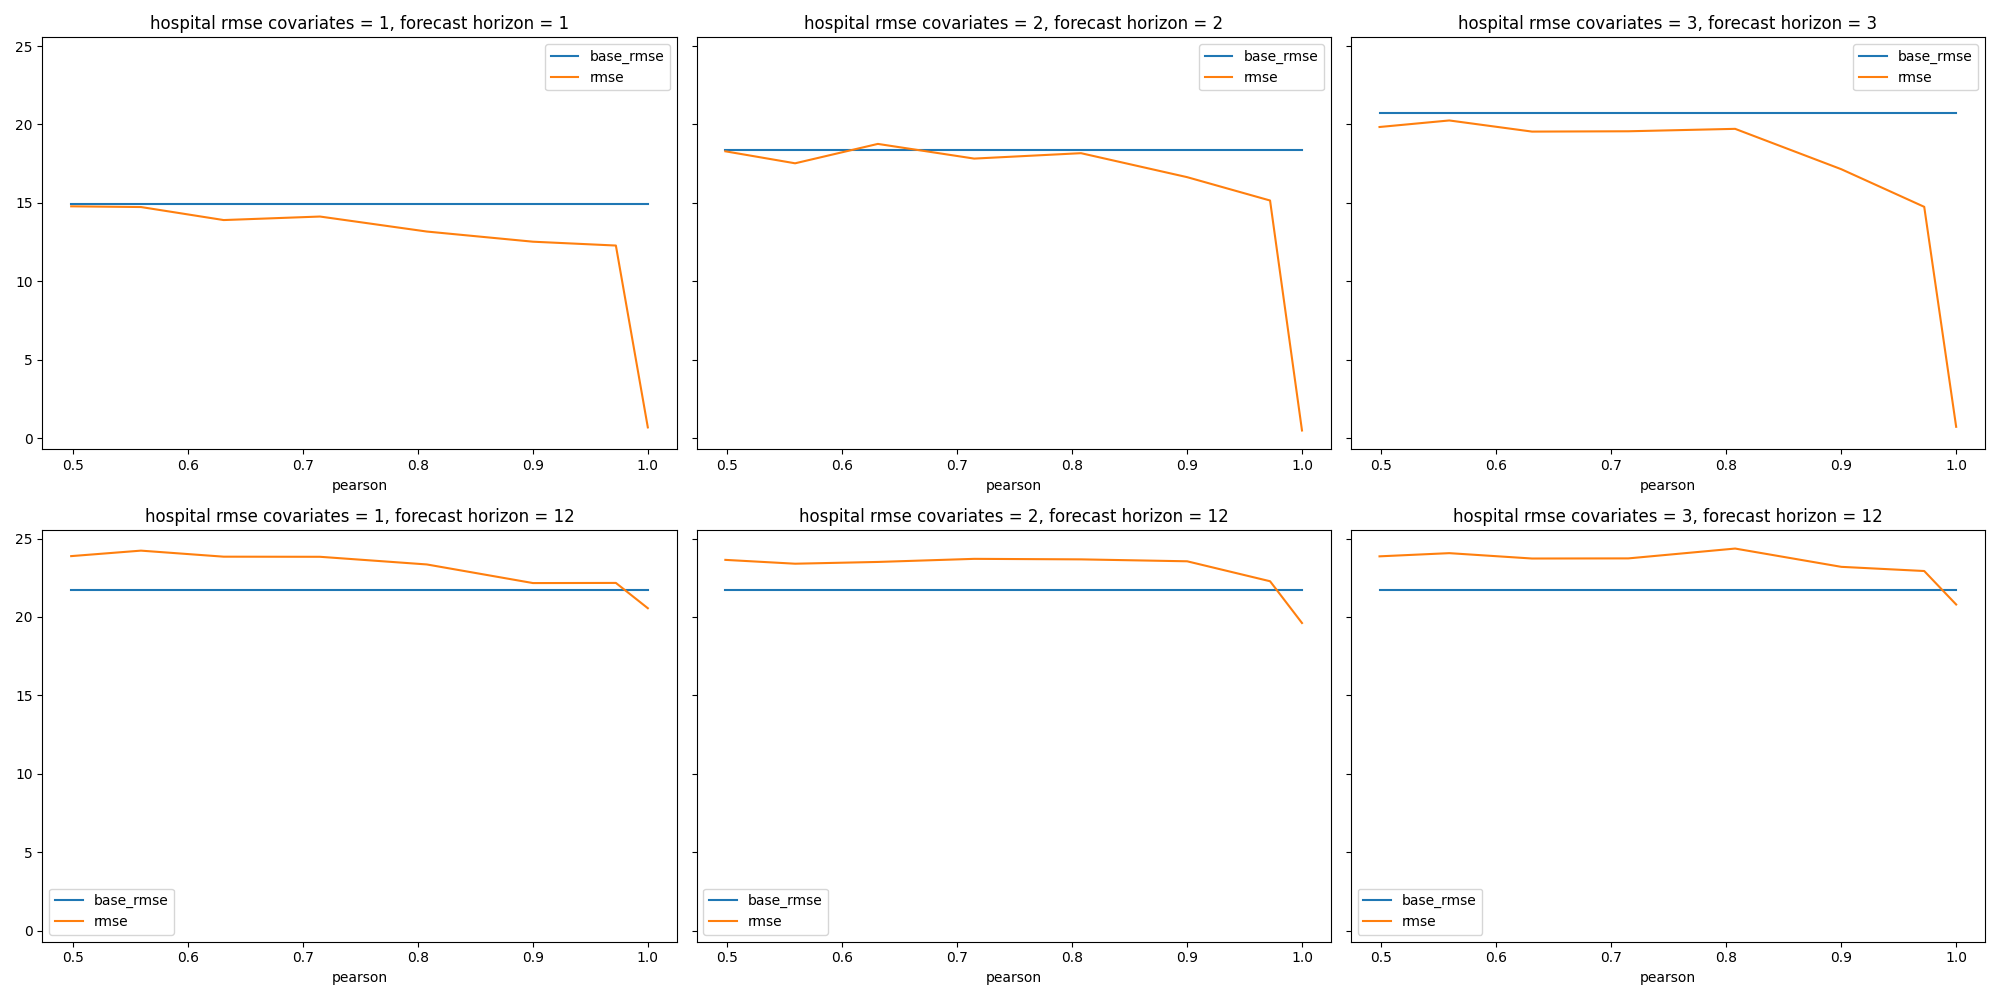
\includegraphics[width=0.9\textwidth]{figures/hospital-base-lstm-rmse.png}
\caption{base-lstm Hospital rmse as a function of correlation for 1, 2 and 3 covariates}
\label{fig:base_lstm_hospital_rmse}
\end{figure}

\subsection{Hospital seg-lstm plots}
\begin{figure}[htbp]
\centering
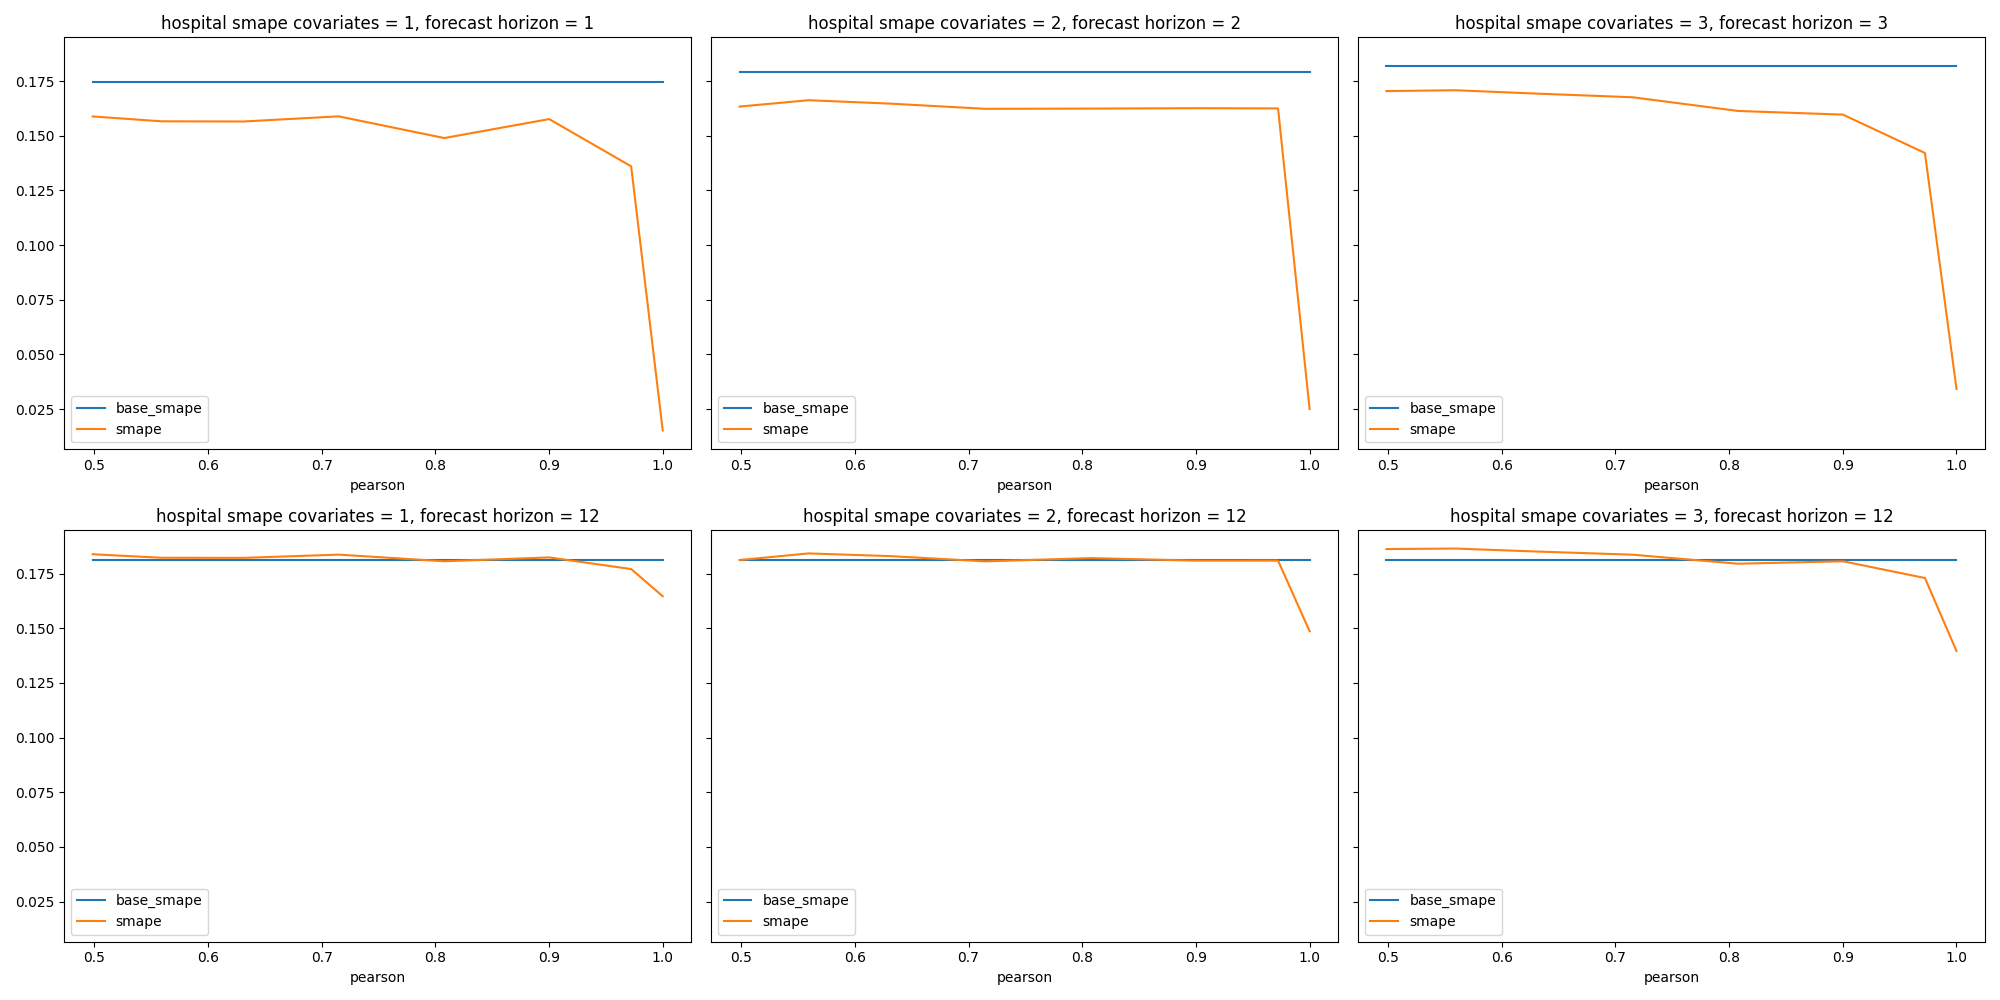
\includegraphics[width=0.9\textwidth]{figures/hospital-seg-lstm-smape.png}
\caption{seg-lstm Hospital smape as a function of correlation for 1, 2 and 3 covariates}
\label{fig:seg_lstm_hospital_smape}
\end{figure}

\begin{figure}[ht]
\centering
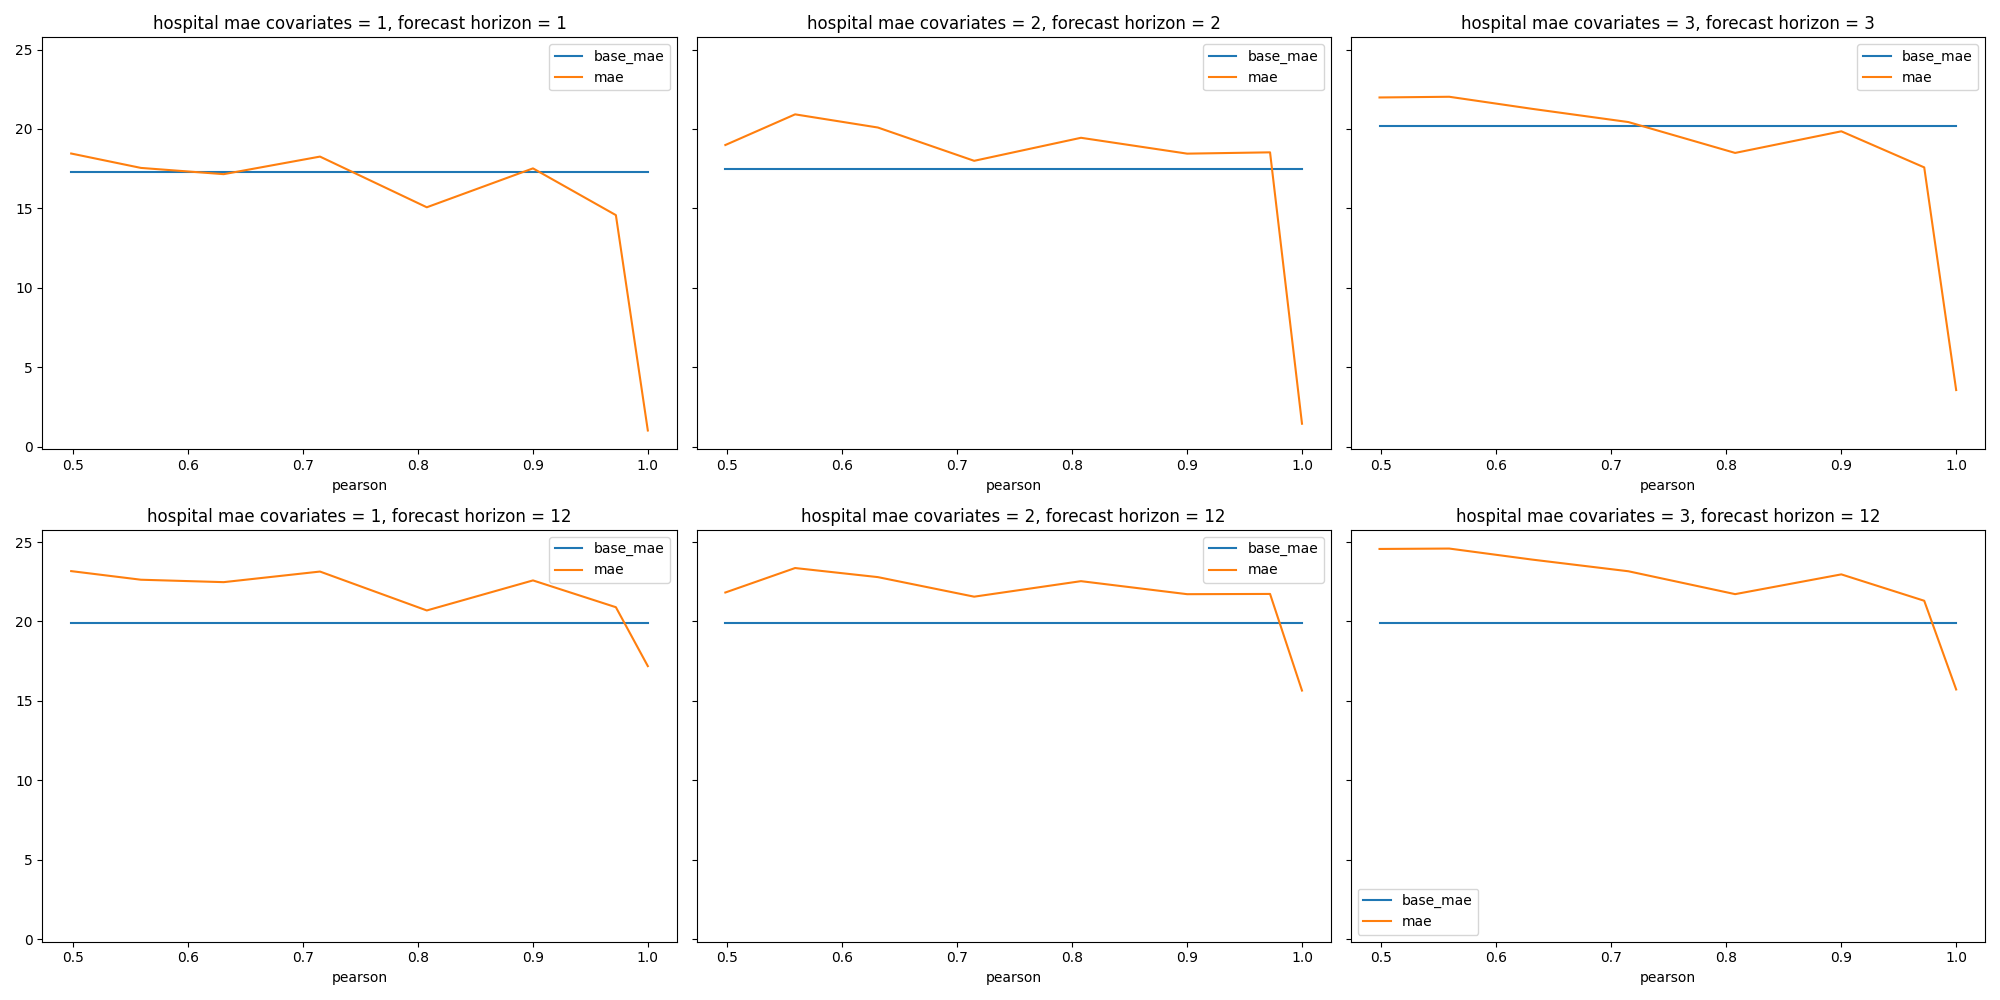
\includegraphics[width=0.9\textwidth]{figures/hospital-seg-lstm-mae.png}
\caption{seg-lstm Hospital mae as a function of correlation for 1, 2 and 3 covariates}
\label{fig:seg_lstm_hospital_mae}
\end{figure}

\begin{figure}[ht]
\centering
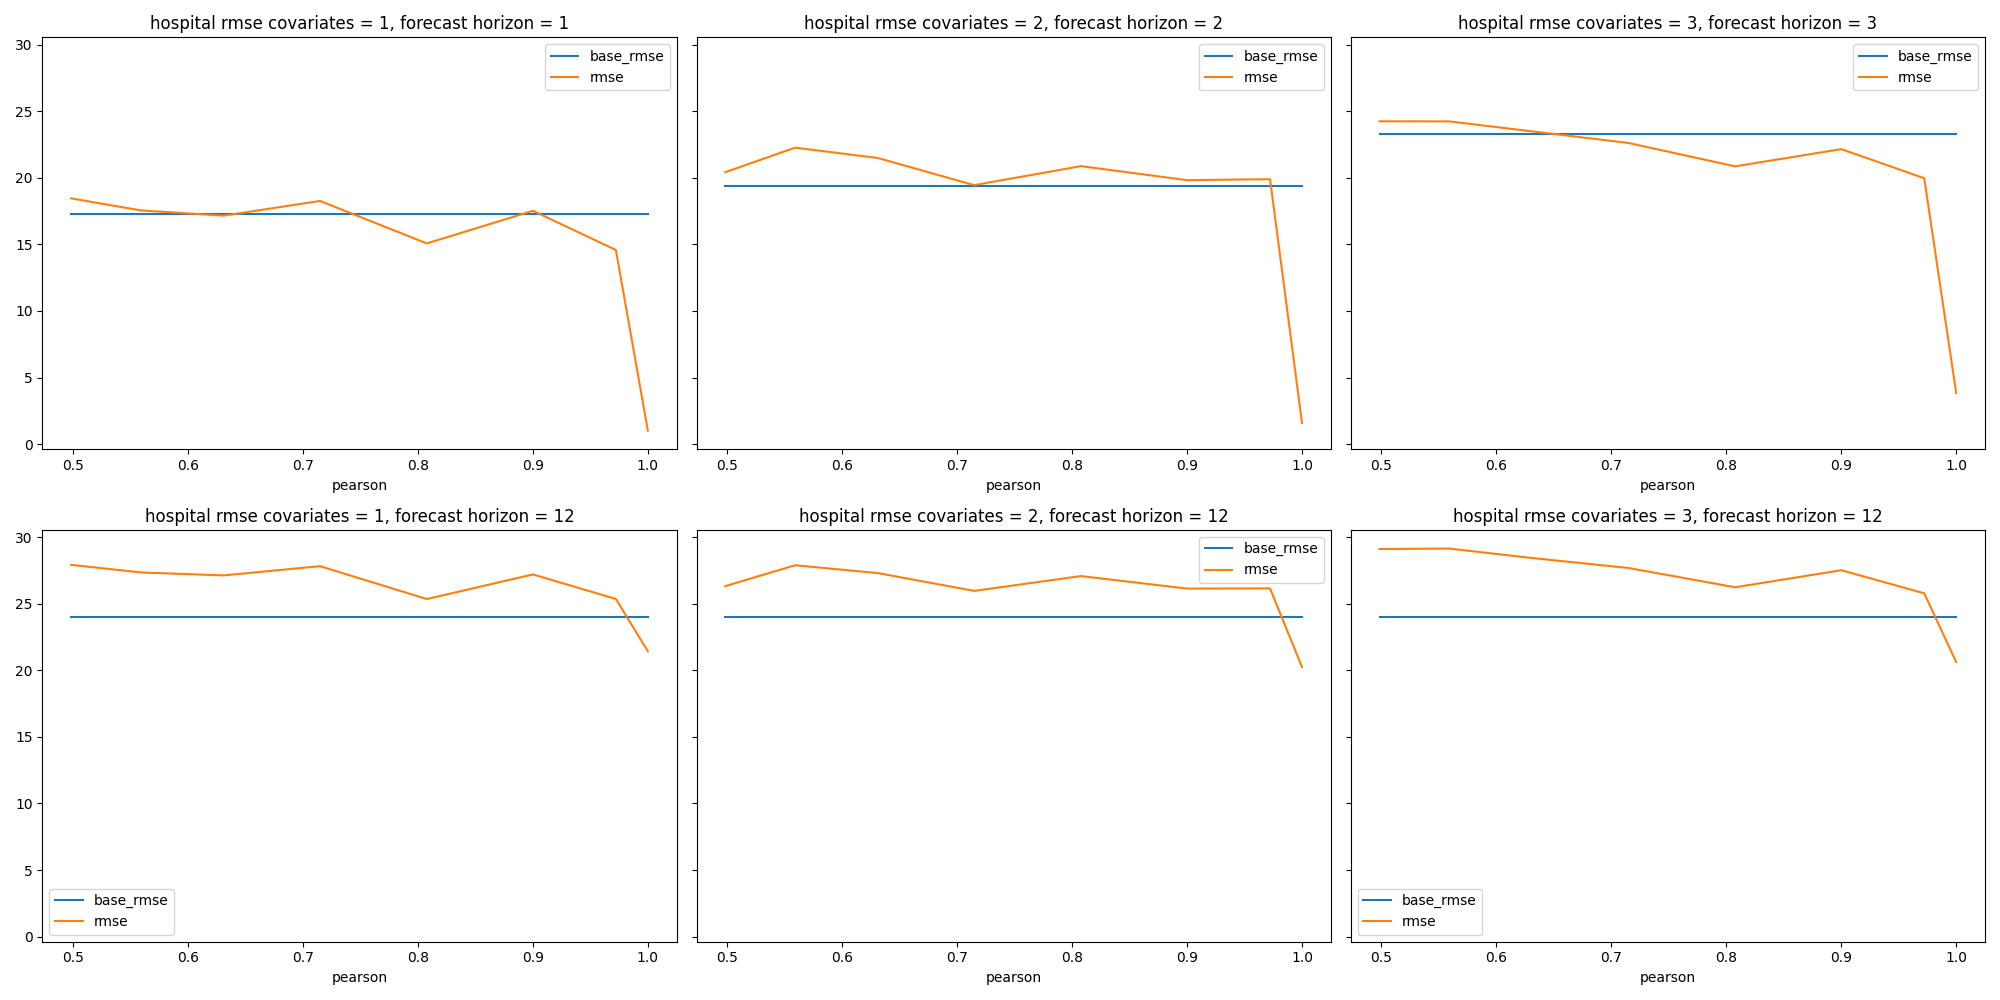
\includegraphics[width=0.9\textwidth]{figures/hospital-seg-lstm-rmse.png}
\caption{seg-lstm Hospital rmse as a function of correlation for 1, 2 and 3 covariates}
\label{fig:seg_lstm_hospital_rmse}
\end{figure}
  


\subsection{tourism}
\begin{figure}[htb]
  \centering
  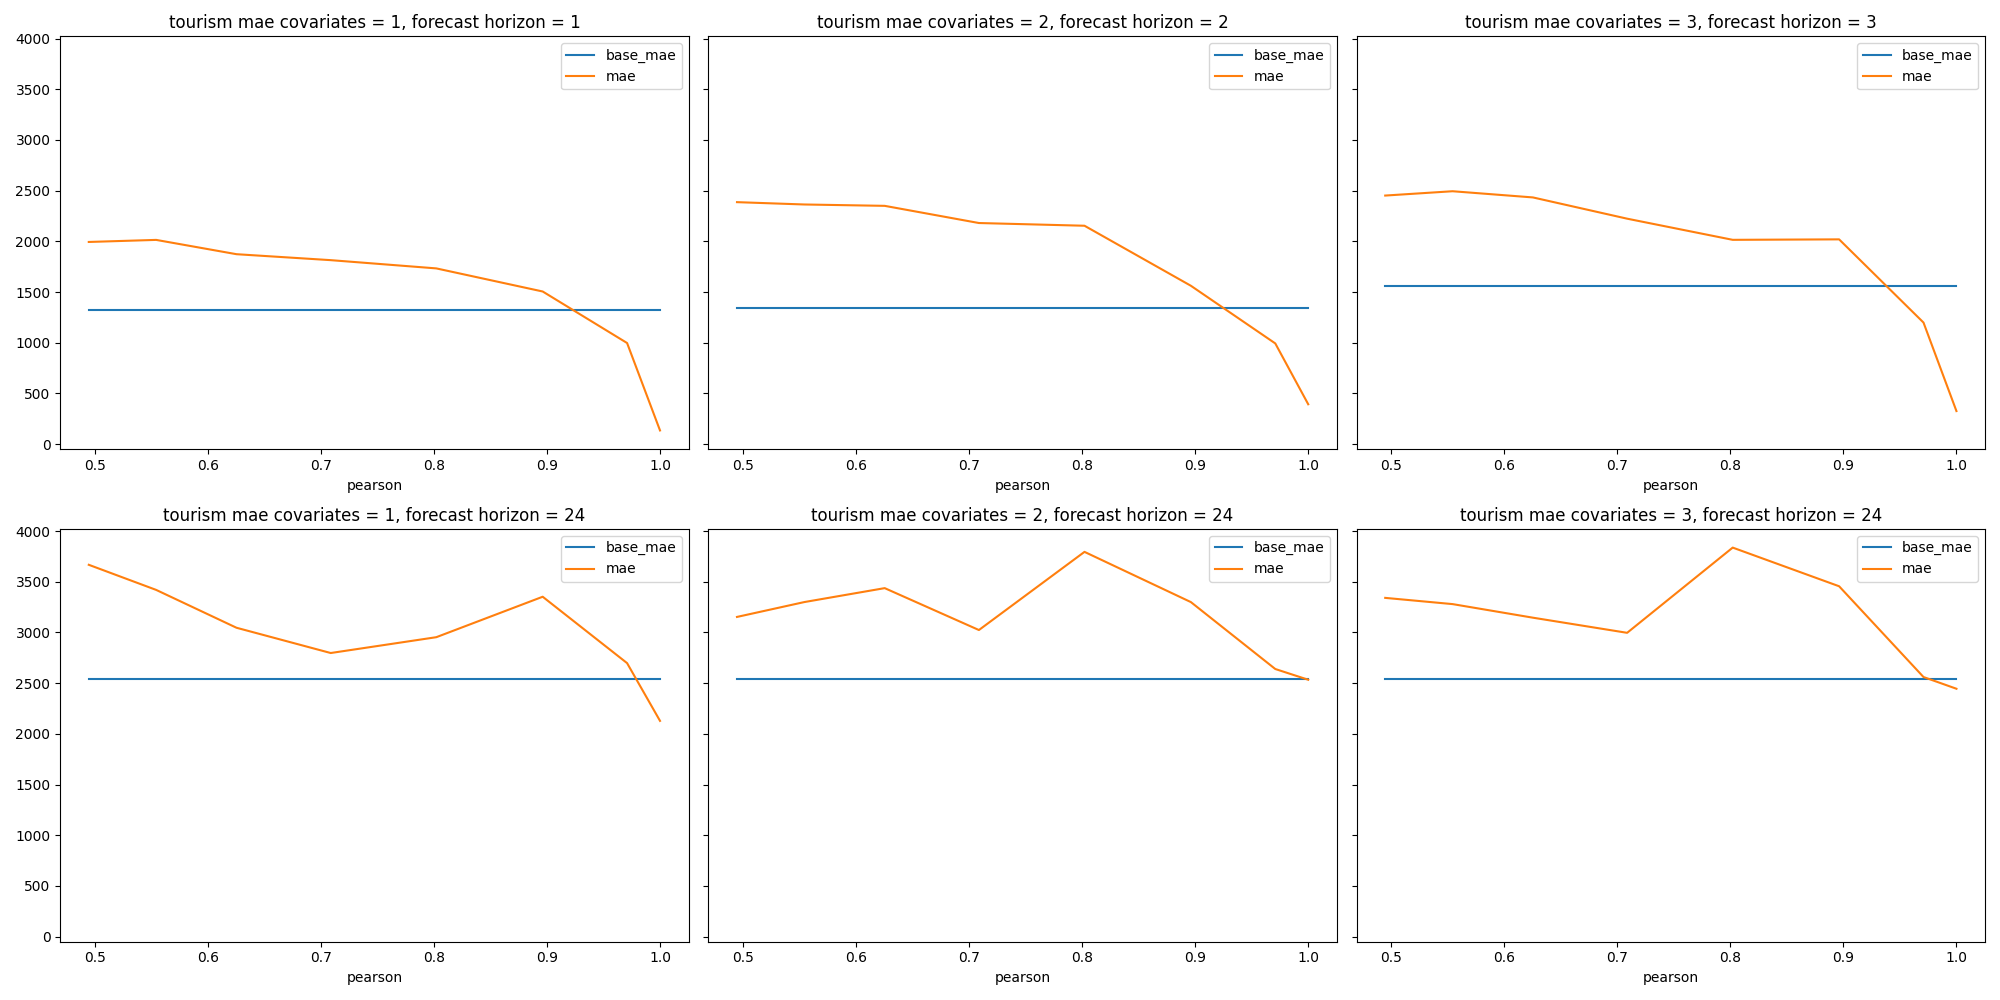
\includegraphics[width=0.9\textwidth]{figures/tourism-base-lstm-mae.png}
  \caption{base-lstm Tourism mae as a function of correlation for 1, 2 and 3 covariates}
  \label{fig:base_lstm_tourism_mae}
  \end{figure}
  
  \begin{figure}[ht]
  \centering
  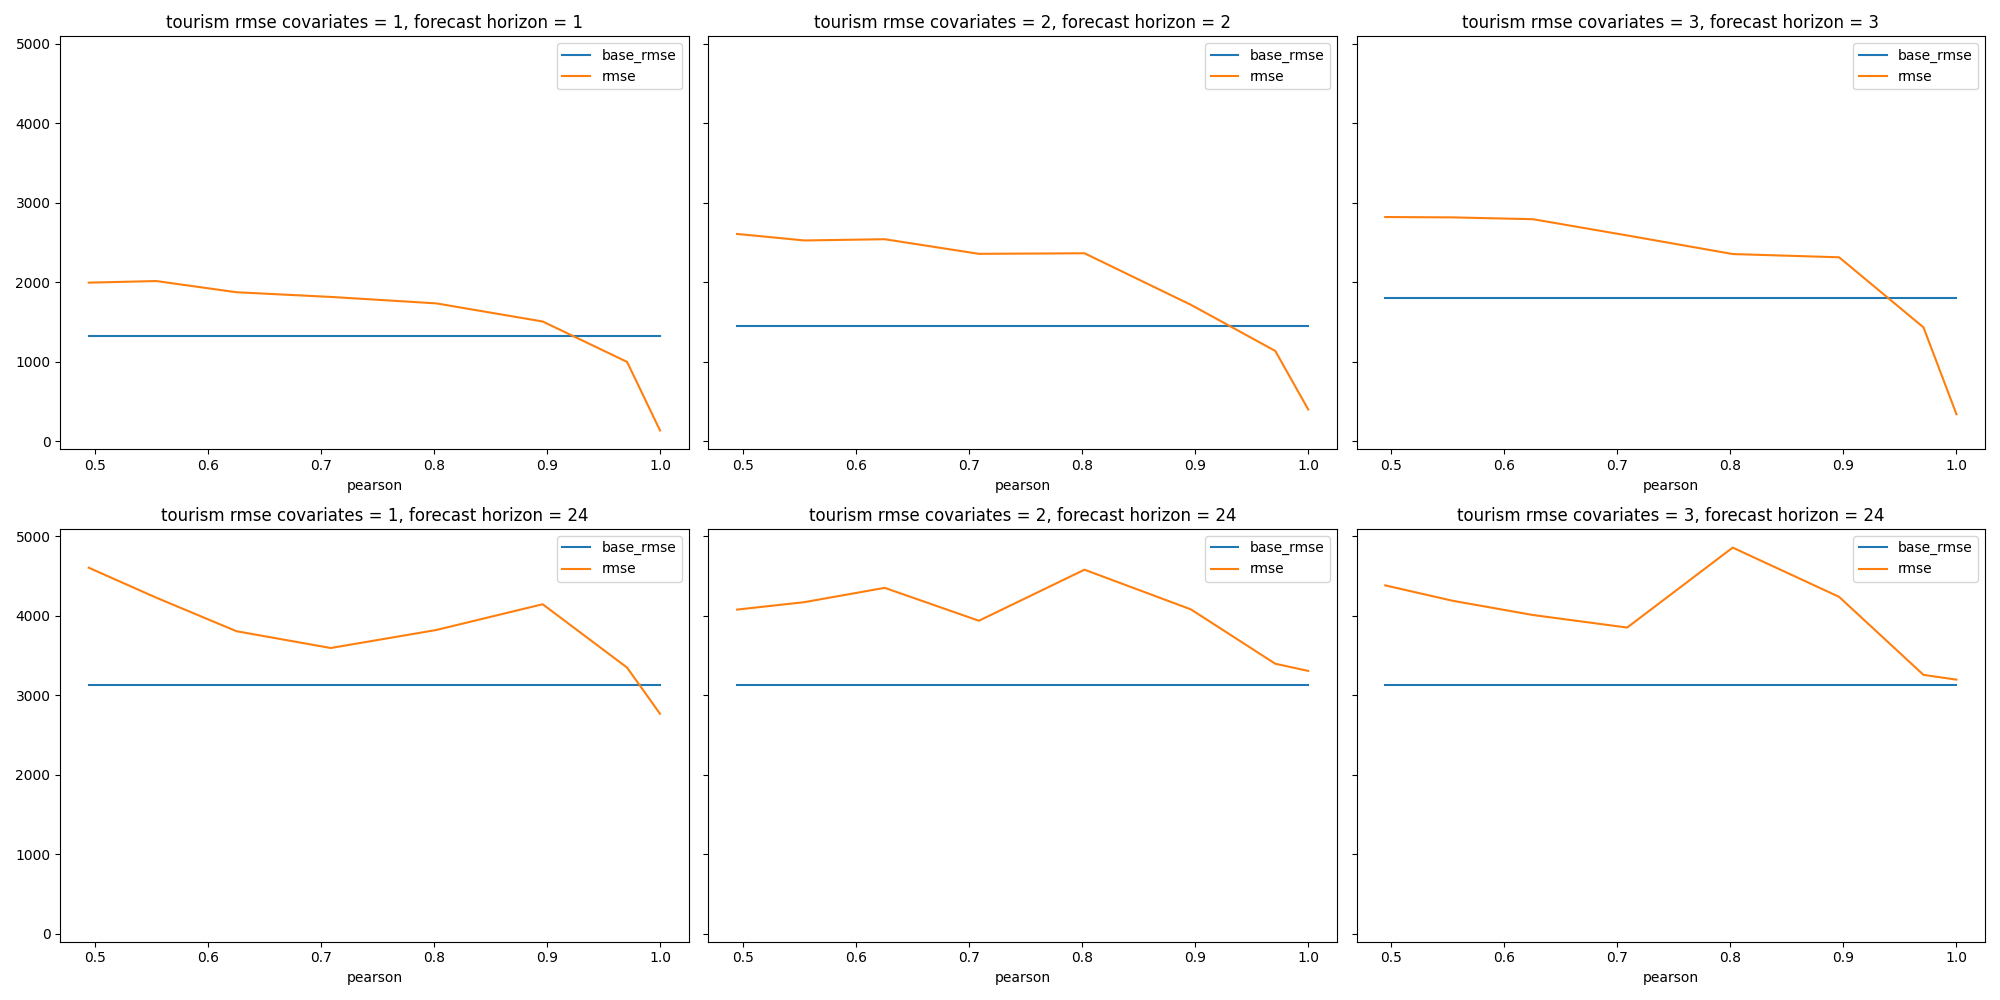
\includegraphics[width=0.9\textwidth]{figures/tourism-base-lstm-rmse.png}
  \caption{base-lstm Tourism rmse as a function of correlation for 1, 2 and 3 covariates}
  \label{fig:base_lstm_tourism_rmse}
  \end{figure}

  \begin{figure}[ht]
  \centering
  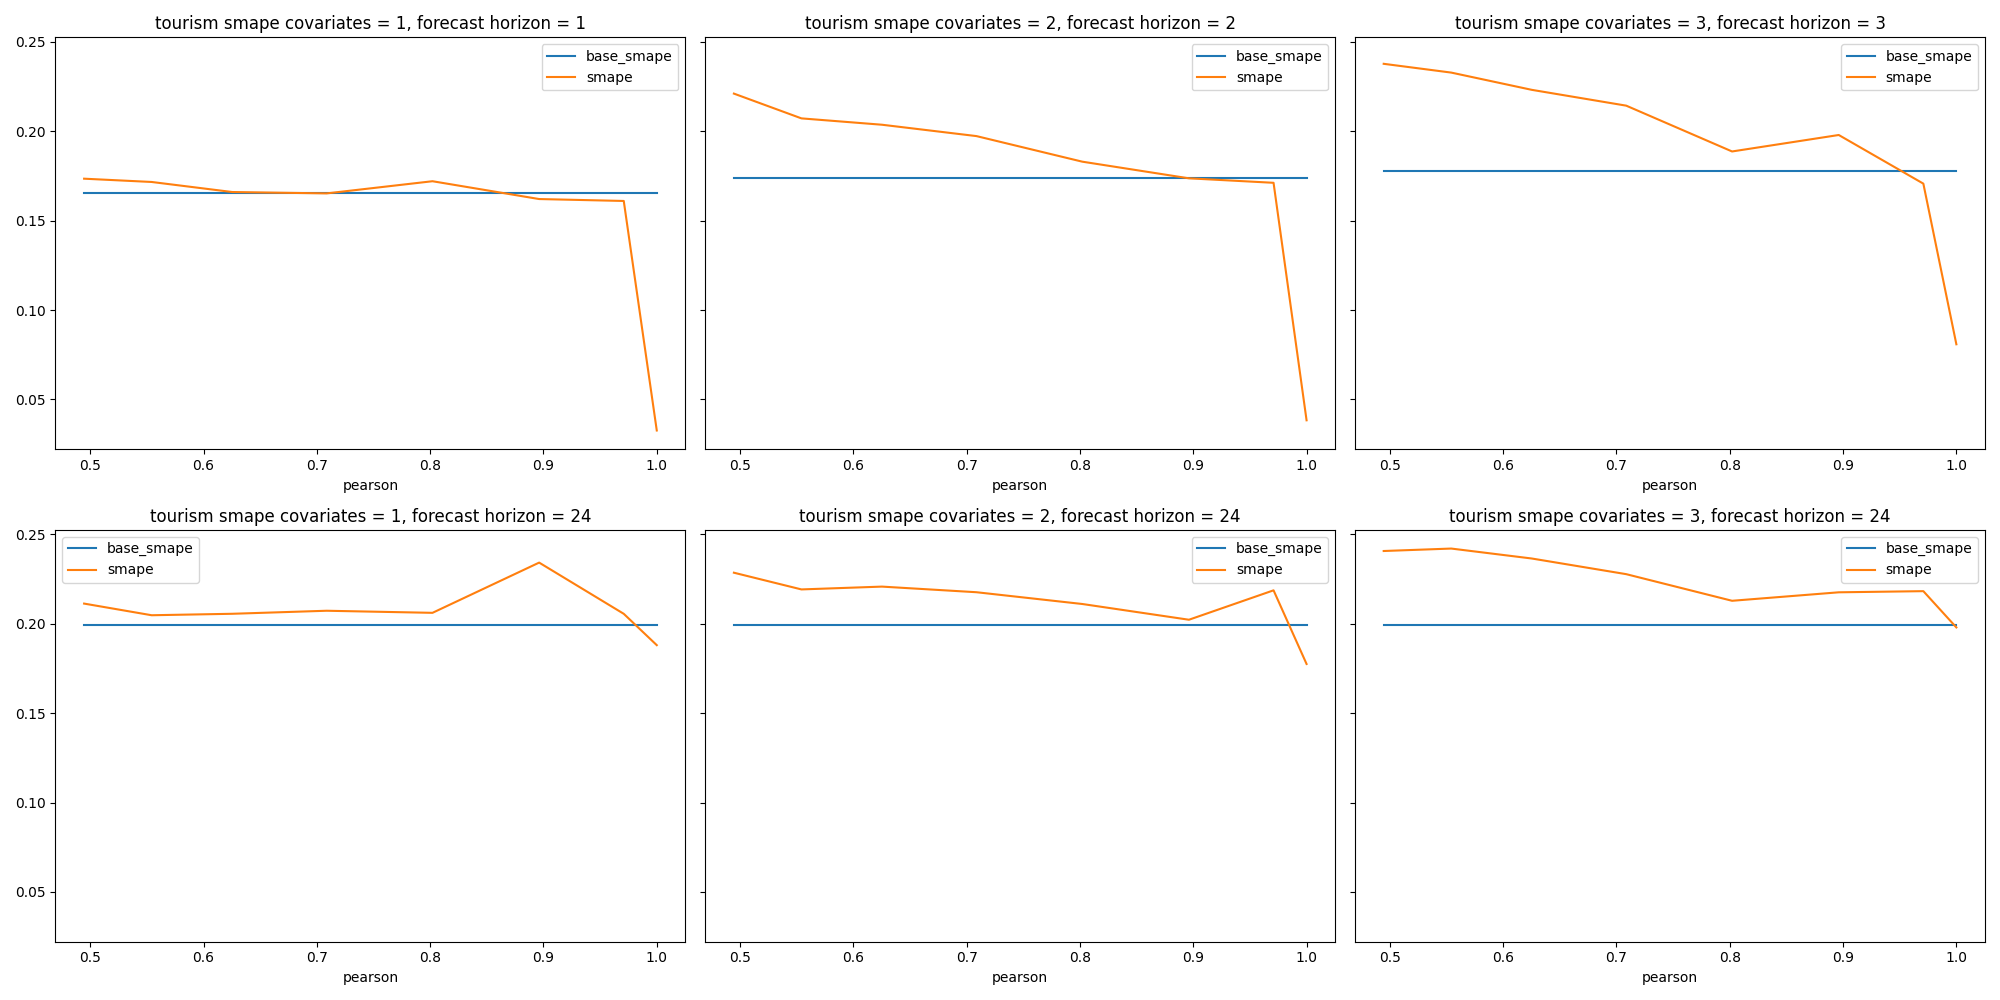
\includegraphics[width=0.9\textwidth]{figures/tourism-seg-lstm-smape.png}
  \caption{seg-lstm Tourism smape as a function of correlation for 1, 2 and 3 covariates}
  \label{fig:seg_lstm_tourism_smape}
  \end{figure}
  
  \begin{figure}[ht]
  \centering
  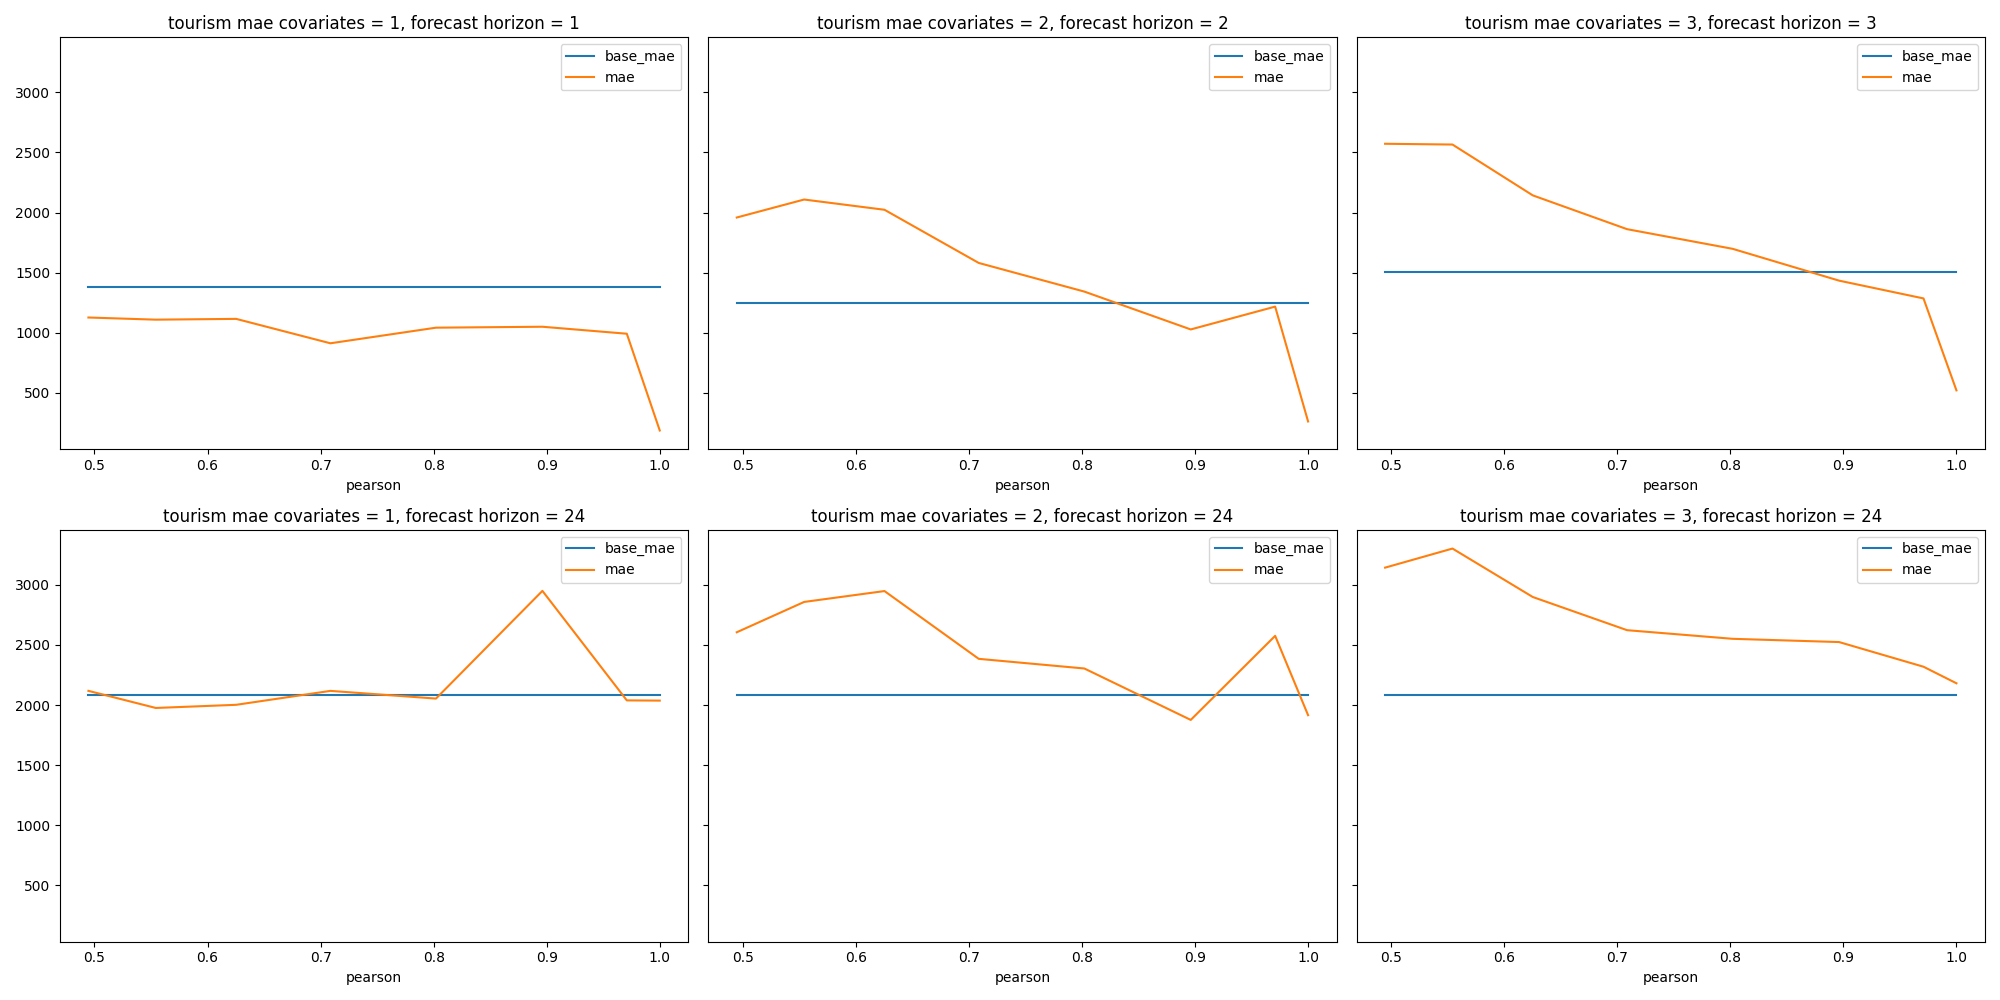
\includegraphics[width=0.9\textwidth]{figures/tourism-seg-lstm-mae.png}
  \caption{seg-lstm Tourism mae as a function of correlation for 1, 2 and 3 covariates}
  \label{fig:seg_lstm_tourism_mae}
  \end{figure}
  
  \begin{figure}[ht]
  \centering
  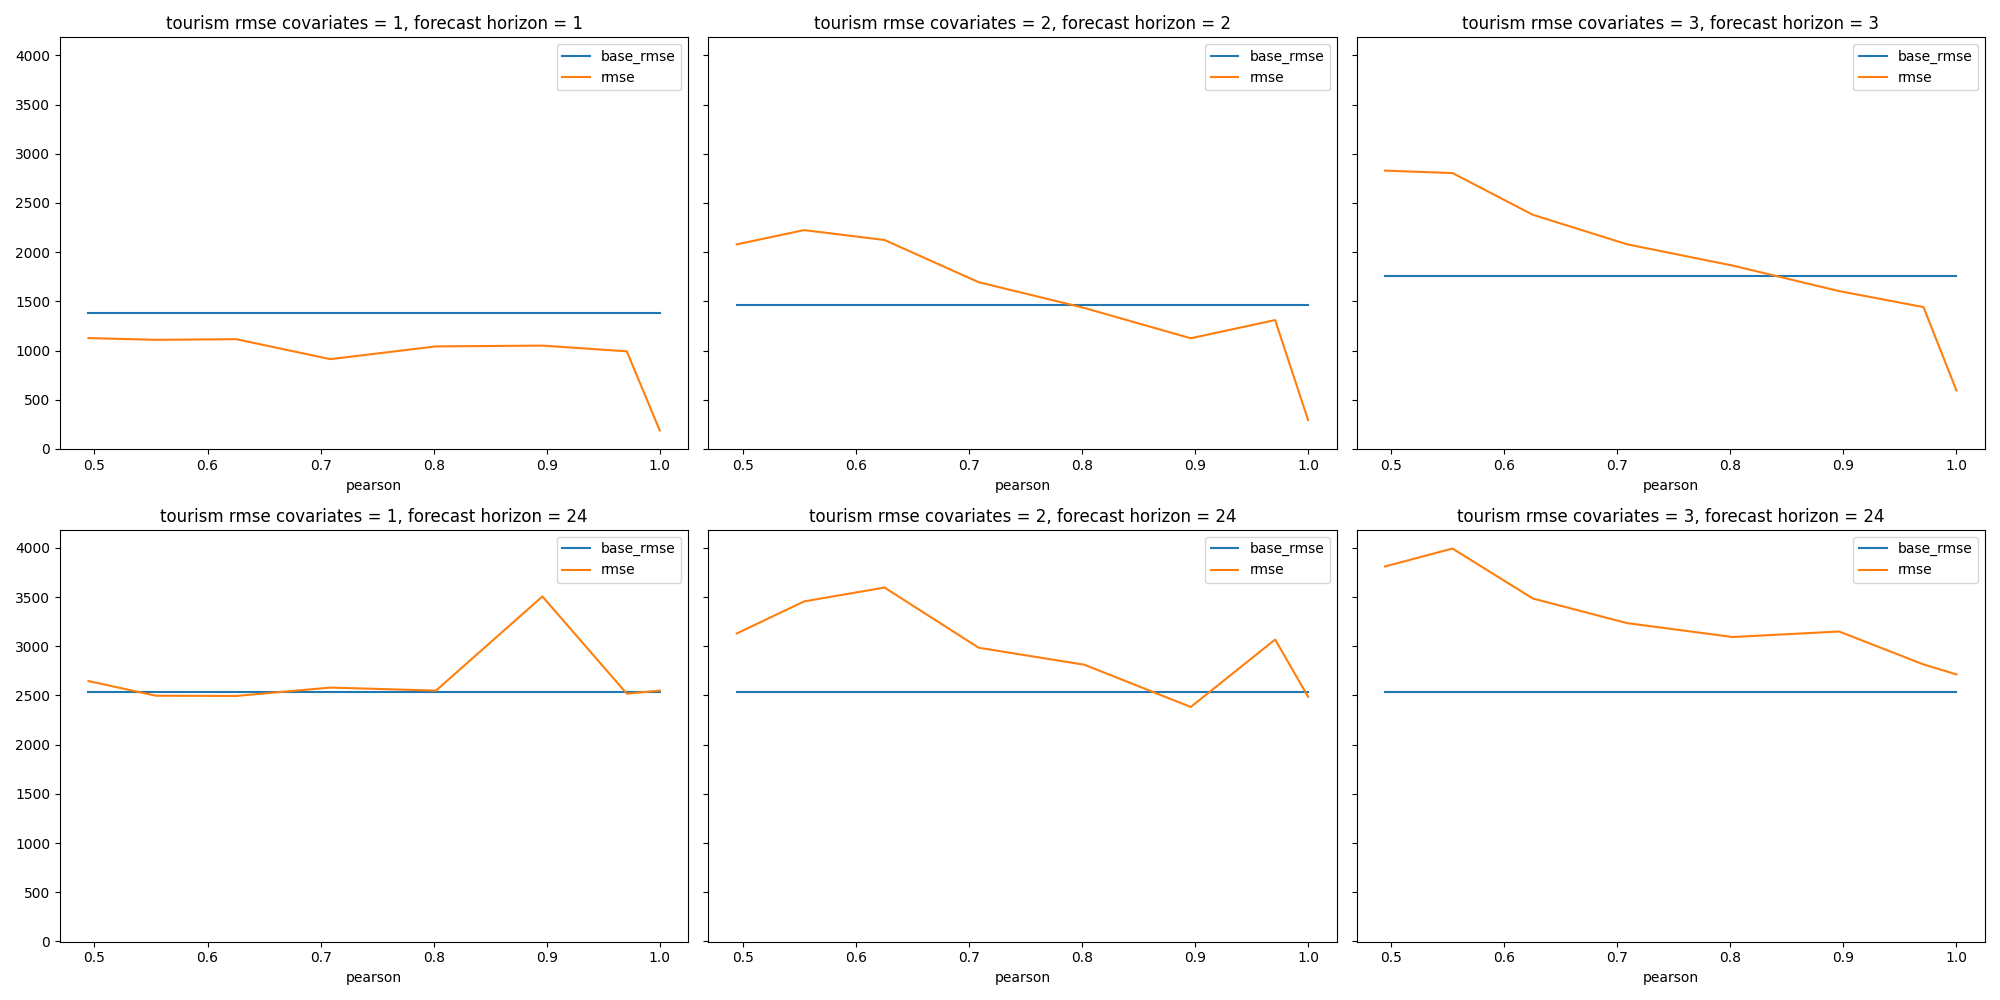
\includegraphics[width=0.9\textwidth]{figures/tourism-seg-lstm-rmse.png}
  \caption{seg-lstm Tourism rmse as a function of correlation for 1, 2 and 3 covariates}
  \label{fig:seg_lstm_tourism_rmse}
  \end{figure}

\subsection{traffic}
  \begin{figure}[htbp]
  \centering
  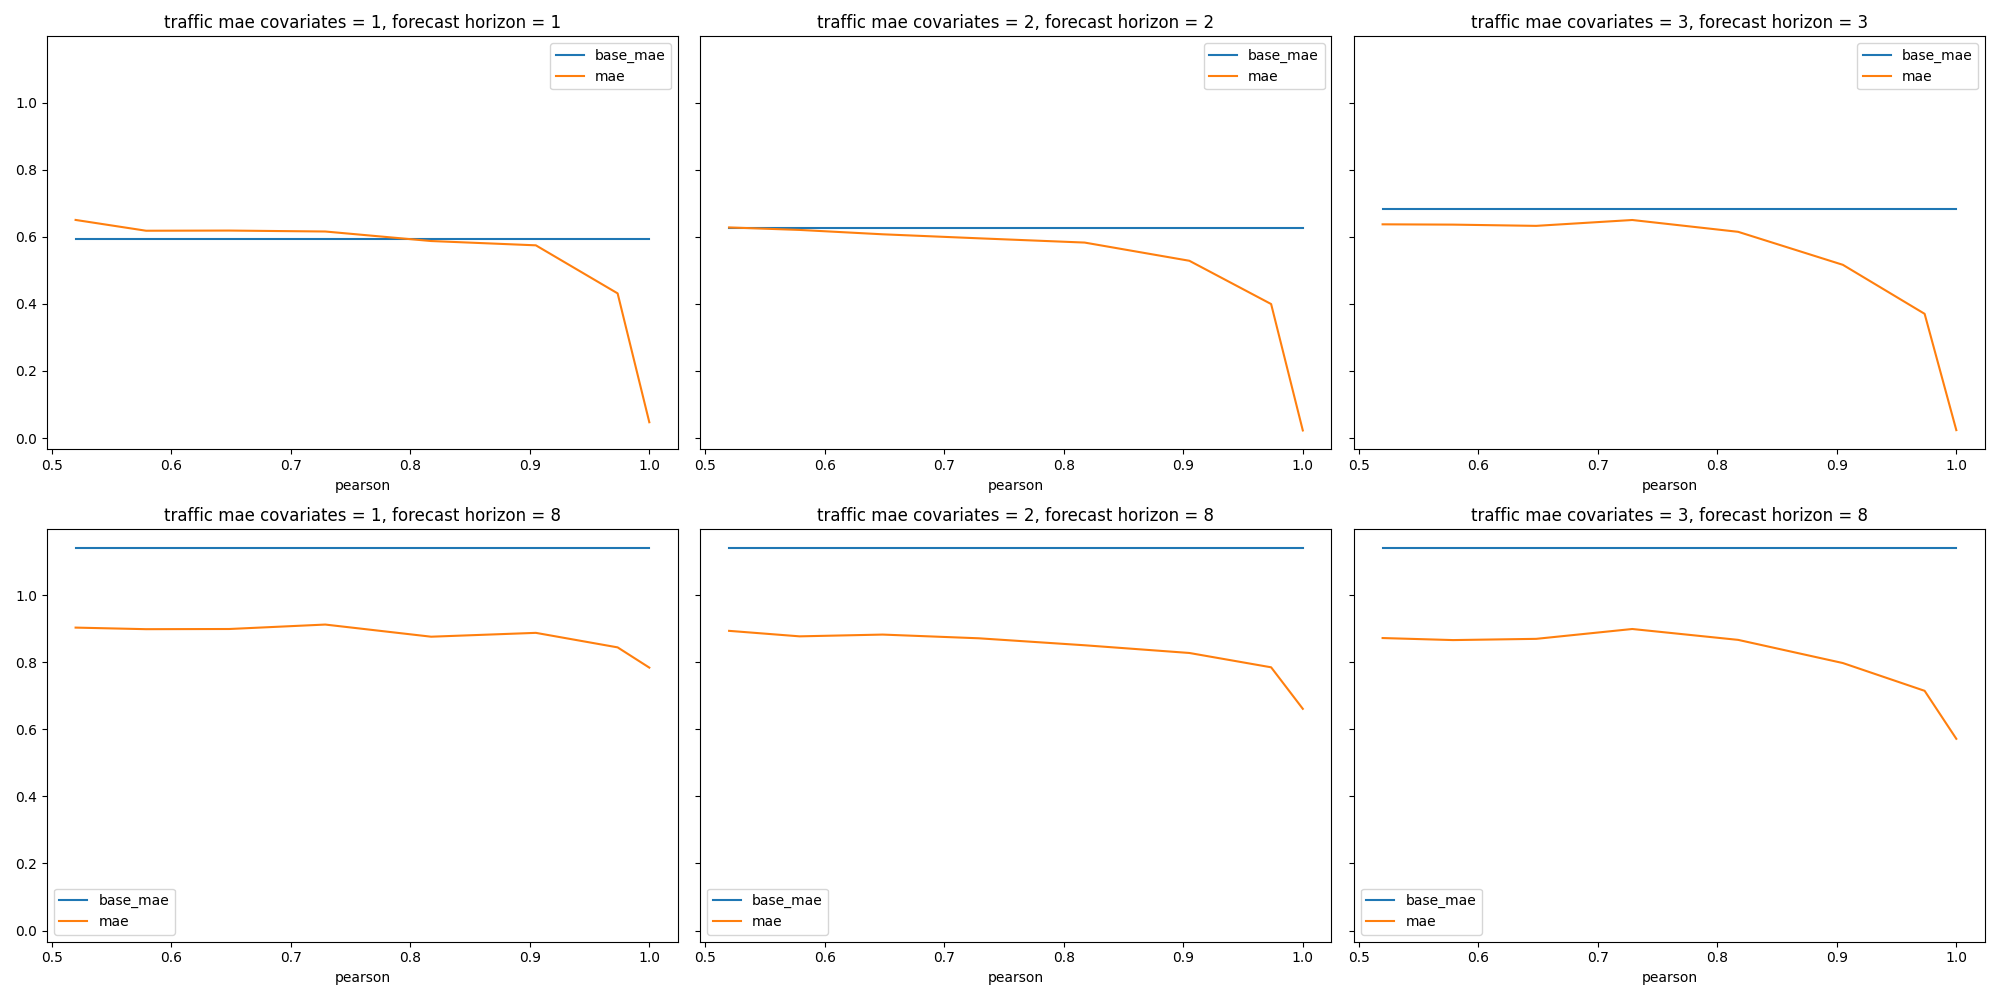
\includegraphics[width=0.9\textwidth]{figures/traffic-base-lstm-mae.png}
  \caption{base-lstm Traffic mae as a function of correlation for 1, 2 and 3 covariates}
  \label{fig:base_lstm_traffic_mae}
  \end{figure}
  
  \begin{figure}[ht]
  \centering
  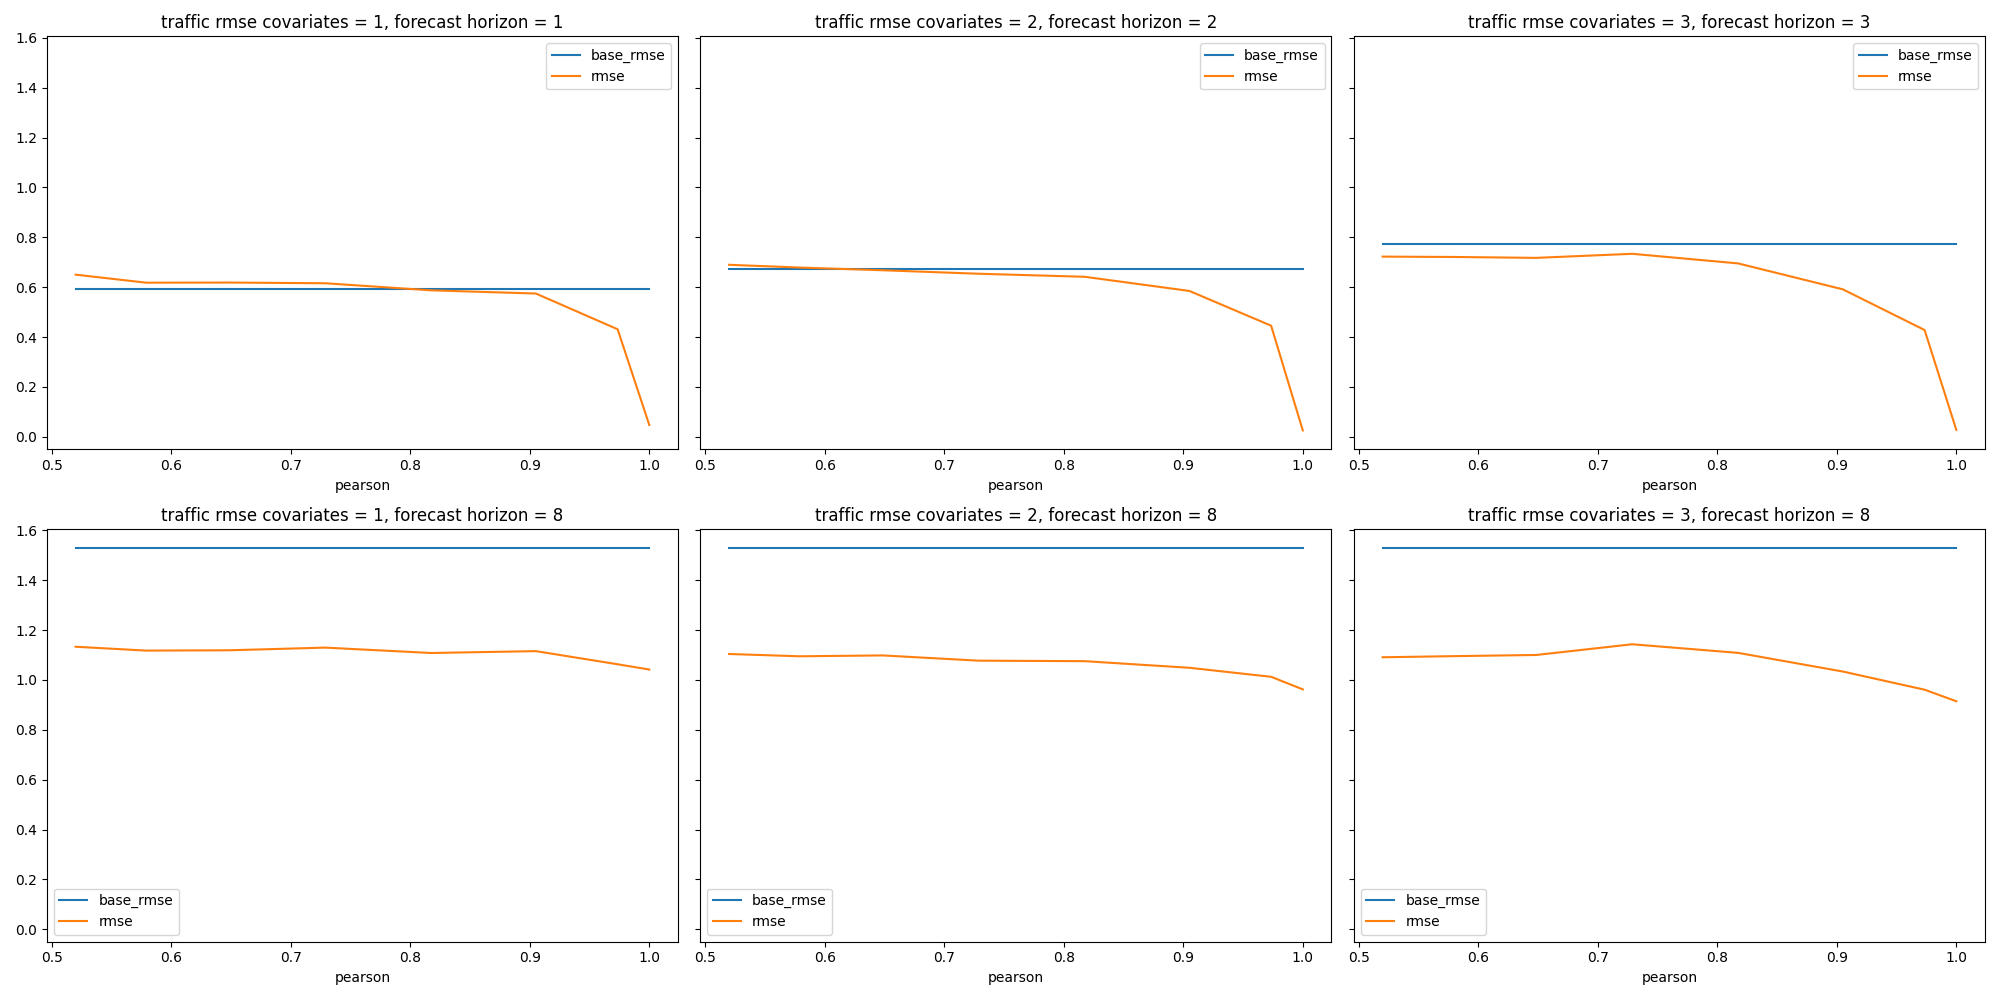
\includegraphics[width=0.9\textwidth]{figures/traffic-base-lstm-rmse.png}
  \caption{base-lstm Traffic rmse as a function of correlation for 1, 2 and 3 covariates}
  \label{fig:base_lstm_traffc_rmse}
  \end{figure}

  \begin{figure}[ht]
  \centering
  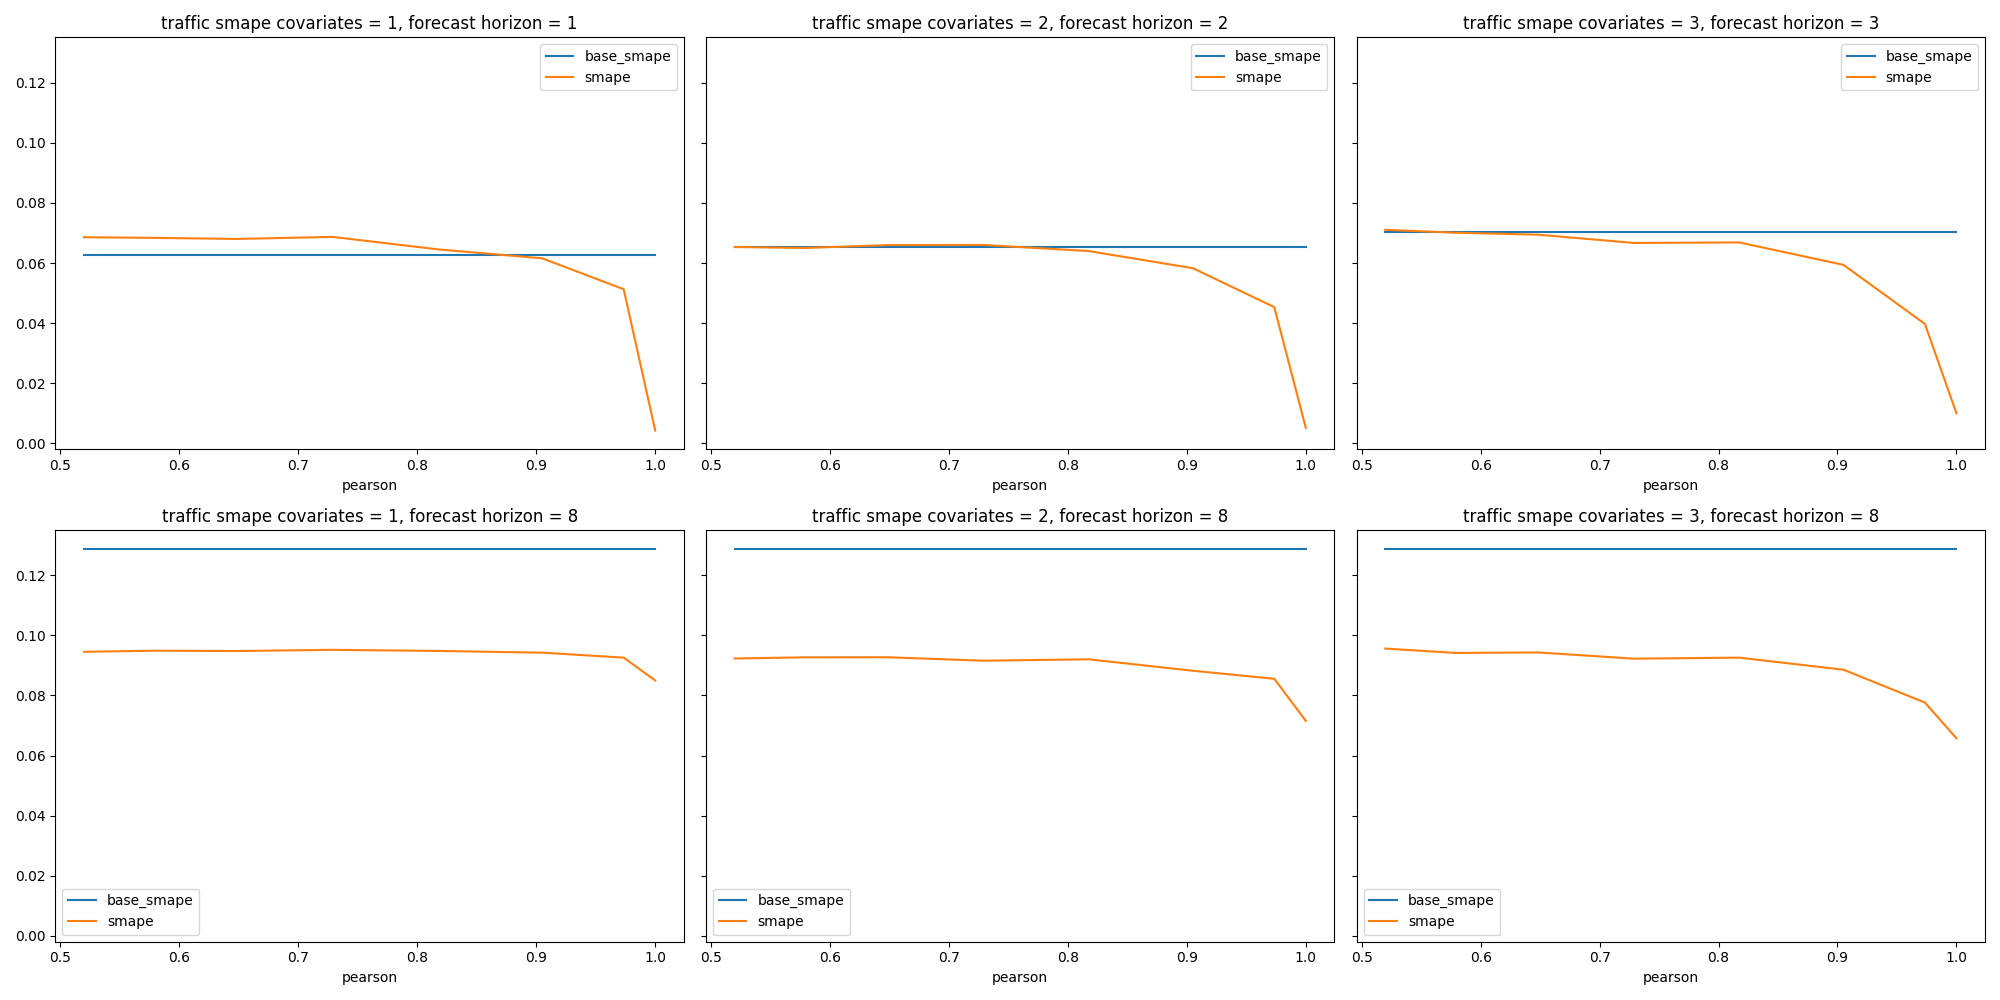
\includegraphics[width=0.9\textwidth]{figures/traffic-seg-lstm-smape.png}
  \caption{seg-lstm Traffic smape as a function of correlation for 1, 2 and 3 covariates}
  \label{fig:seg_lstm_traffic_smape}
  \end{figure}
  
  \begin{figure}[ht]
  \centering
  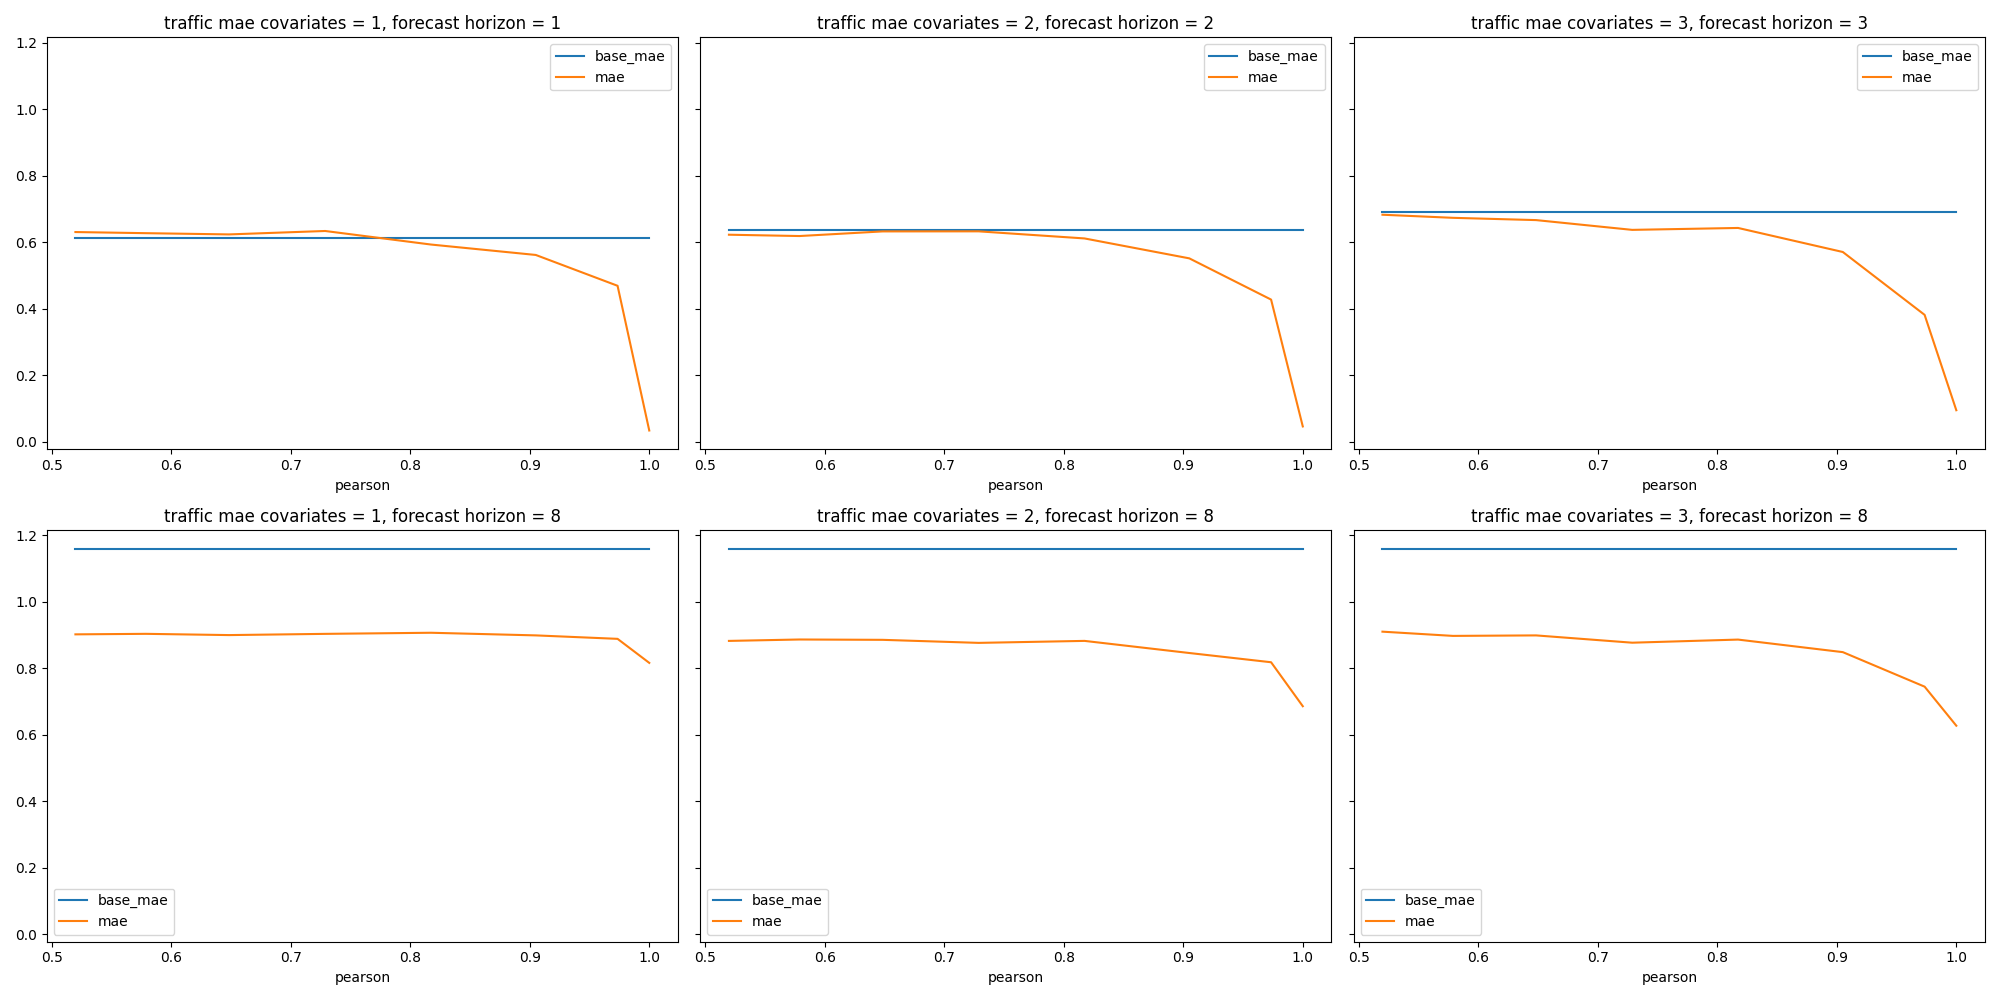
\includegraphics[width=0.9\textwidth]{figures/traffic-seg-lstm-mae.png}
  \caption{seg-lstm Traffic mae as a function of correlation for 1, 2 and 3 covariates}
  \label{fig:seg_lstm_traffic_mae}
  \end{figure}
  
  \begin{figure}[ht]
  \centering
  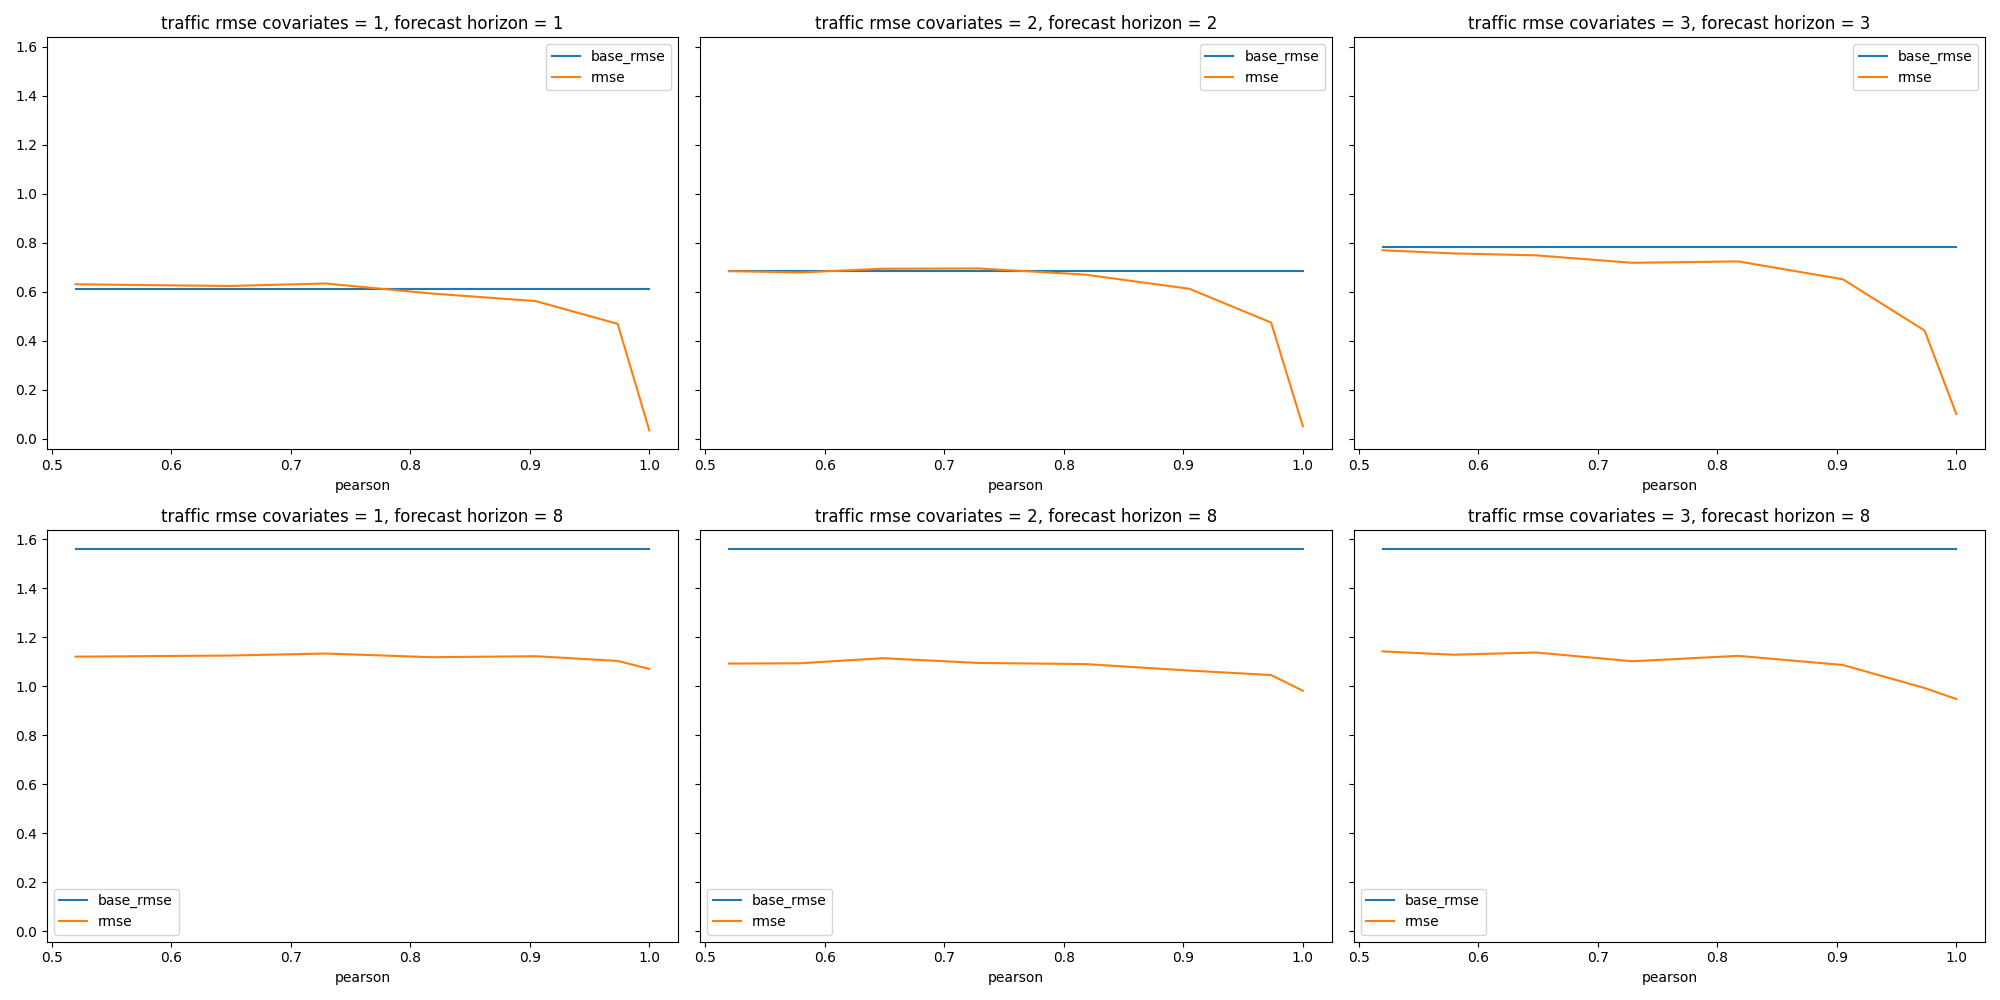
\includegraphics[width=0.9\textwidth]{figures/traffic-seg-lstm-rmse.png}
  \caption{seg-lstm Traffic rmse as a function of correlation for 1, 2 and 3 covariates}
  \label{fig:seg_lstm_traffic_rmse}
  \end{figure}

  \subsection{electricity}
  \begin{figure}[htbp]
  \centering
  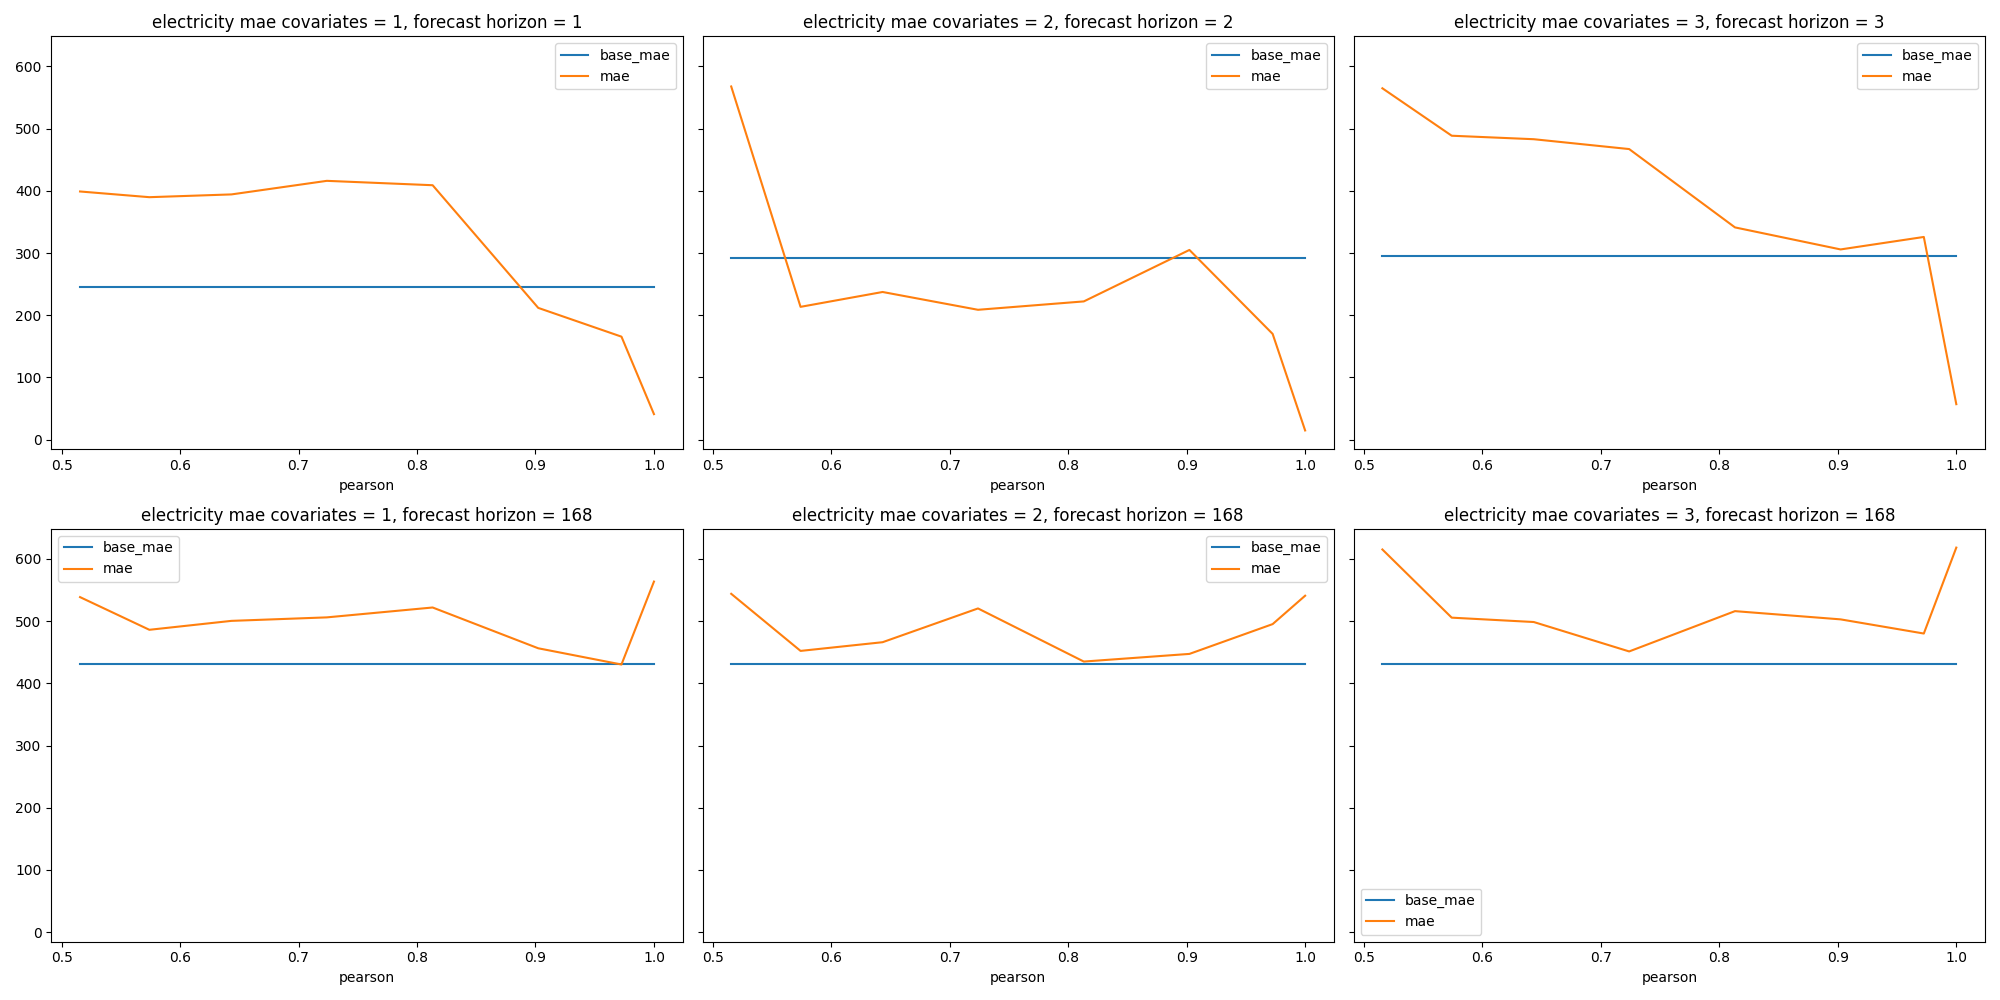
\includegraphics[width=0.9\textwidth]{figures/electricity-base-lstm-mae.png}
  \caption{base-lstm Electricity mae as a function of correlation for 1, 2 and 3 covariates}
  \label{fig:base_lstm_electricity_mae}
  \end{figure}
  
  \begin{figure}[ht]
  \centering
  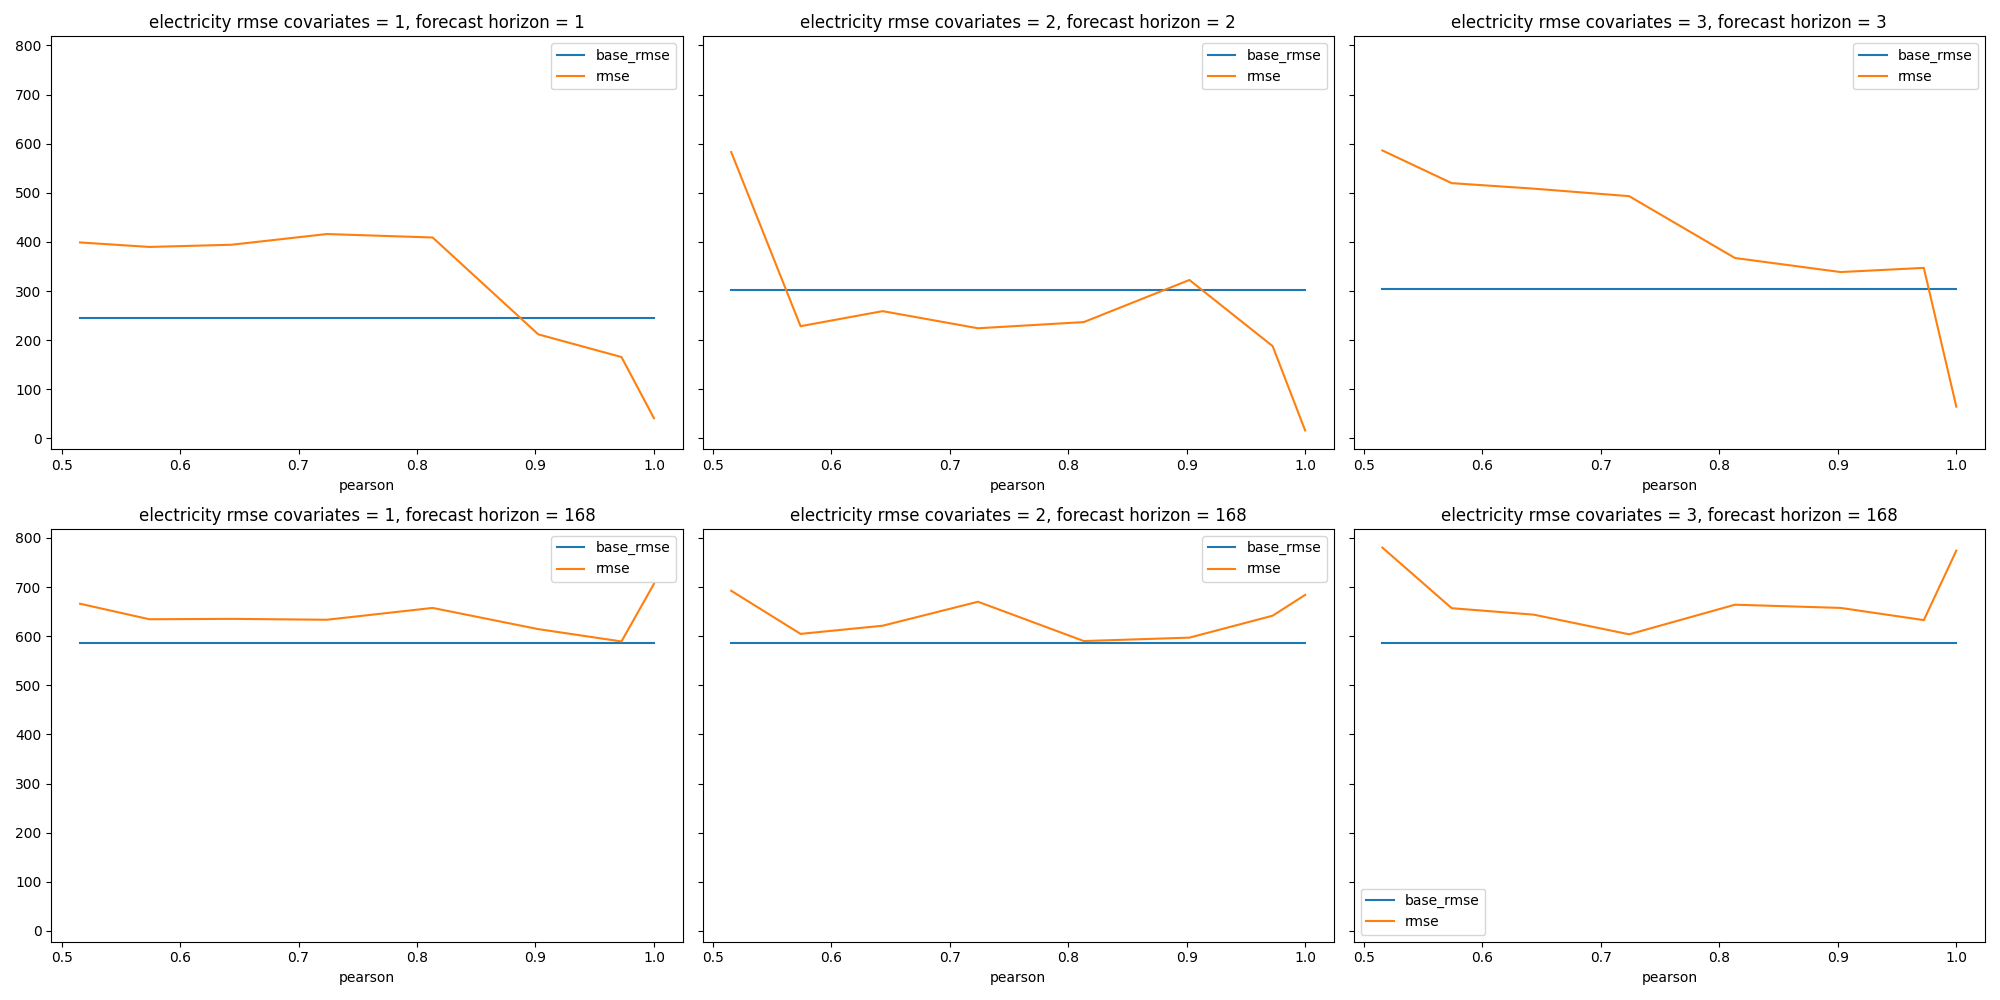
\includegraphics[width=0.9\textwidth]{figures/electricity-base-lstm-rmse.png}
  \caption{base-lstm Electricity rmse as a function of correlation for 1, 2 and 3 covariates}
  \label{fig:base_lstm_electricity_rmse}
  \end{figure}
    
  \begin{figure}[ht]
  \centering
  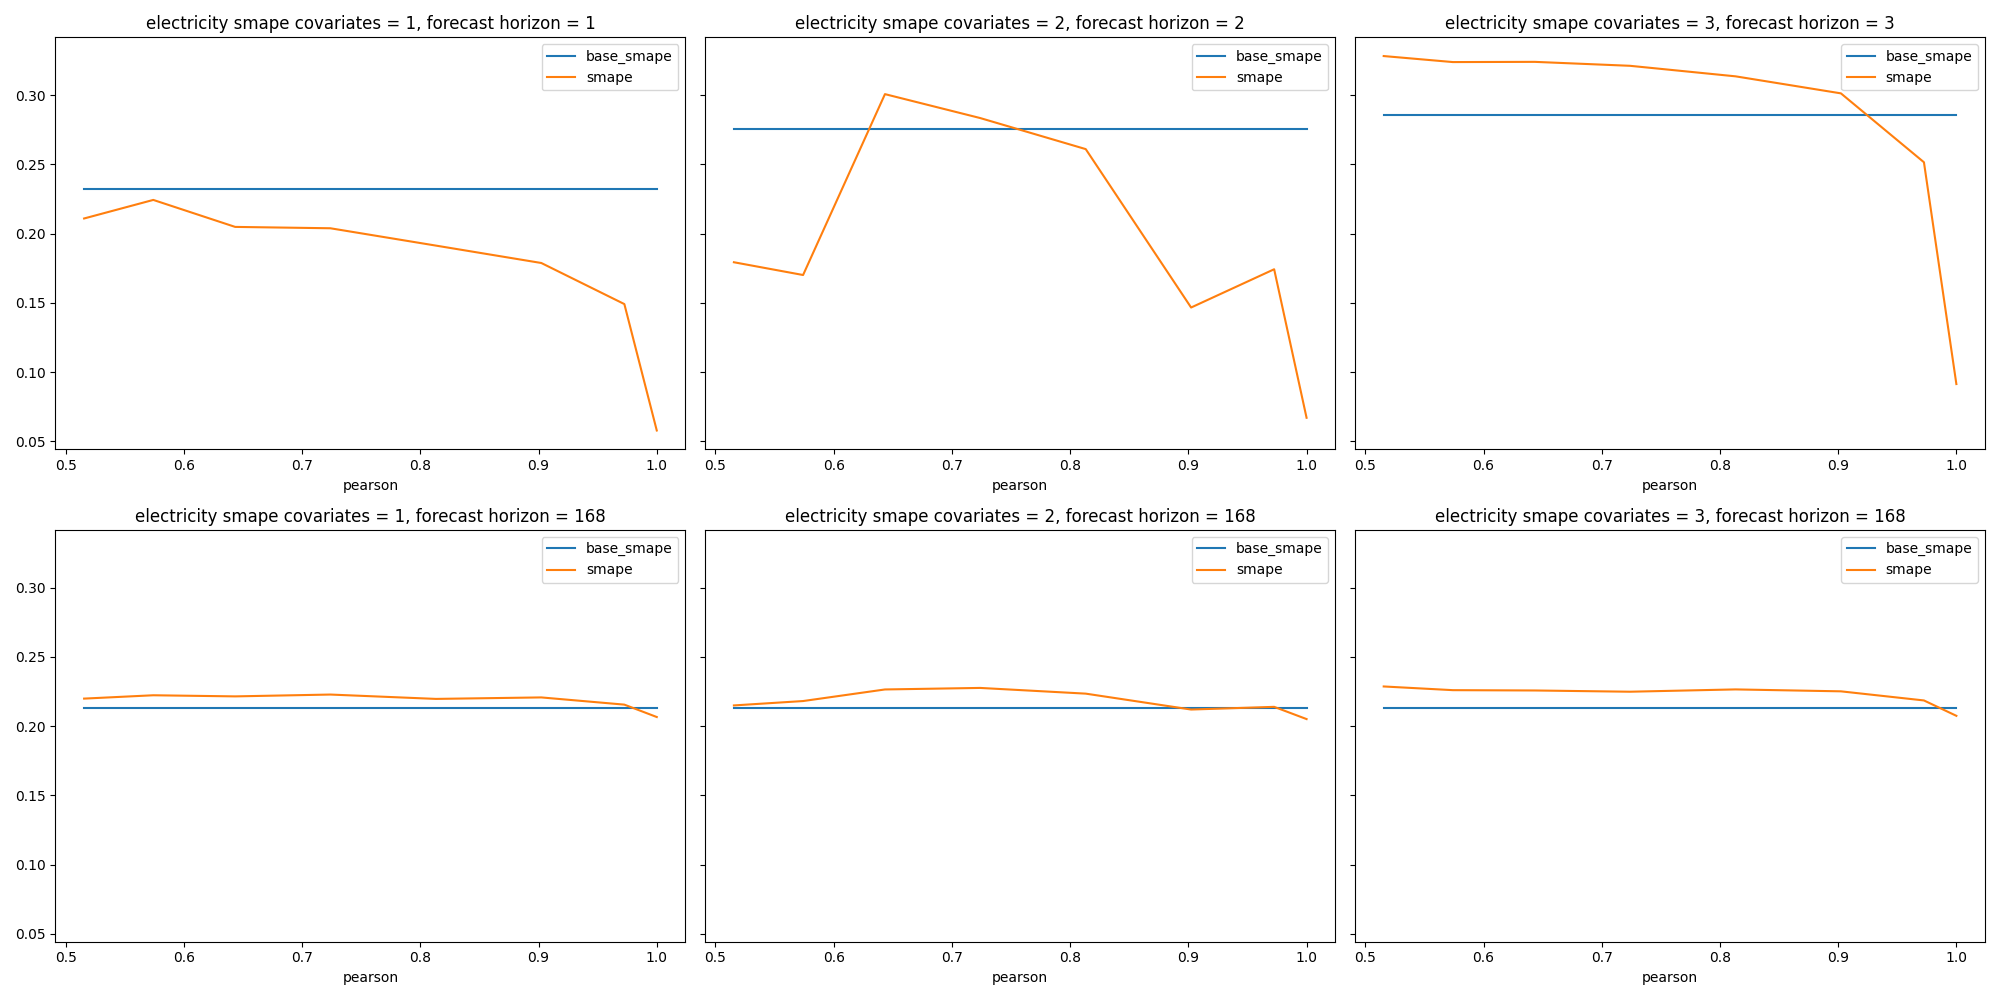
\includegraphics[width=0.9\textwidth]{figures/electricity-seg-lstm-smape.png}
  \caption{seg-lstm Electricity smape as a function of correlation for 1, 2 and 3 covariates}
  \label{fig:seg_lstm_electricity_smape}
  \end{figure}
  
  \begin{figure}[ht]
  \centering
  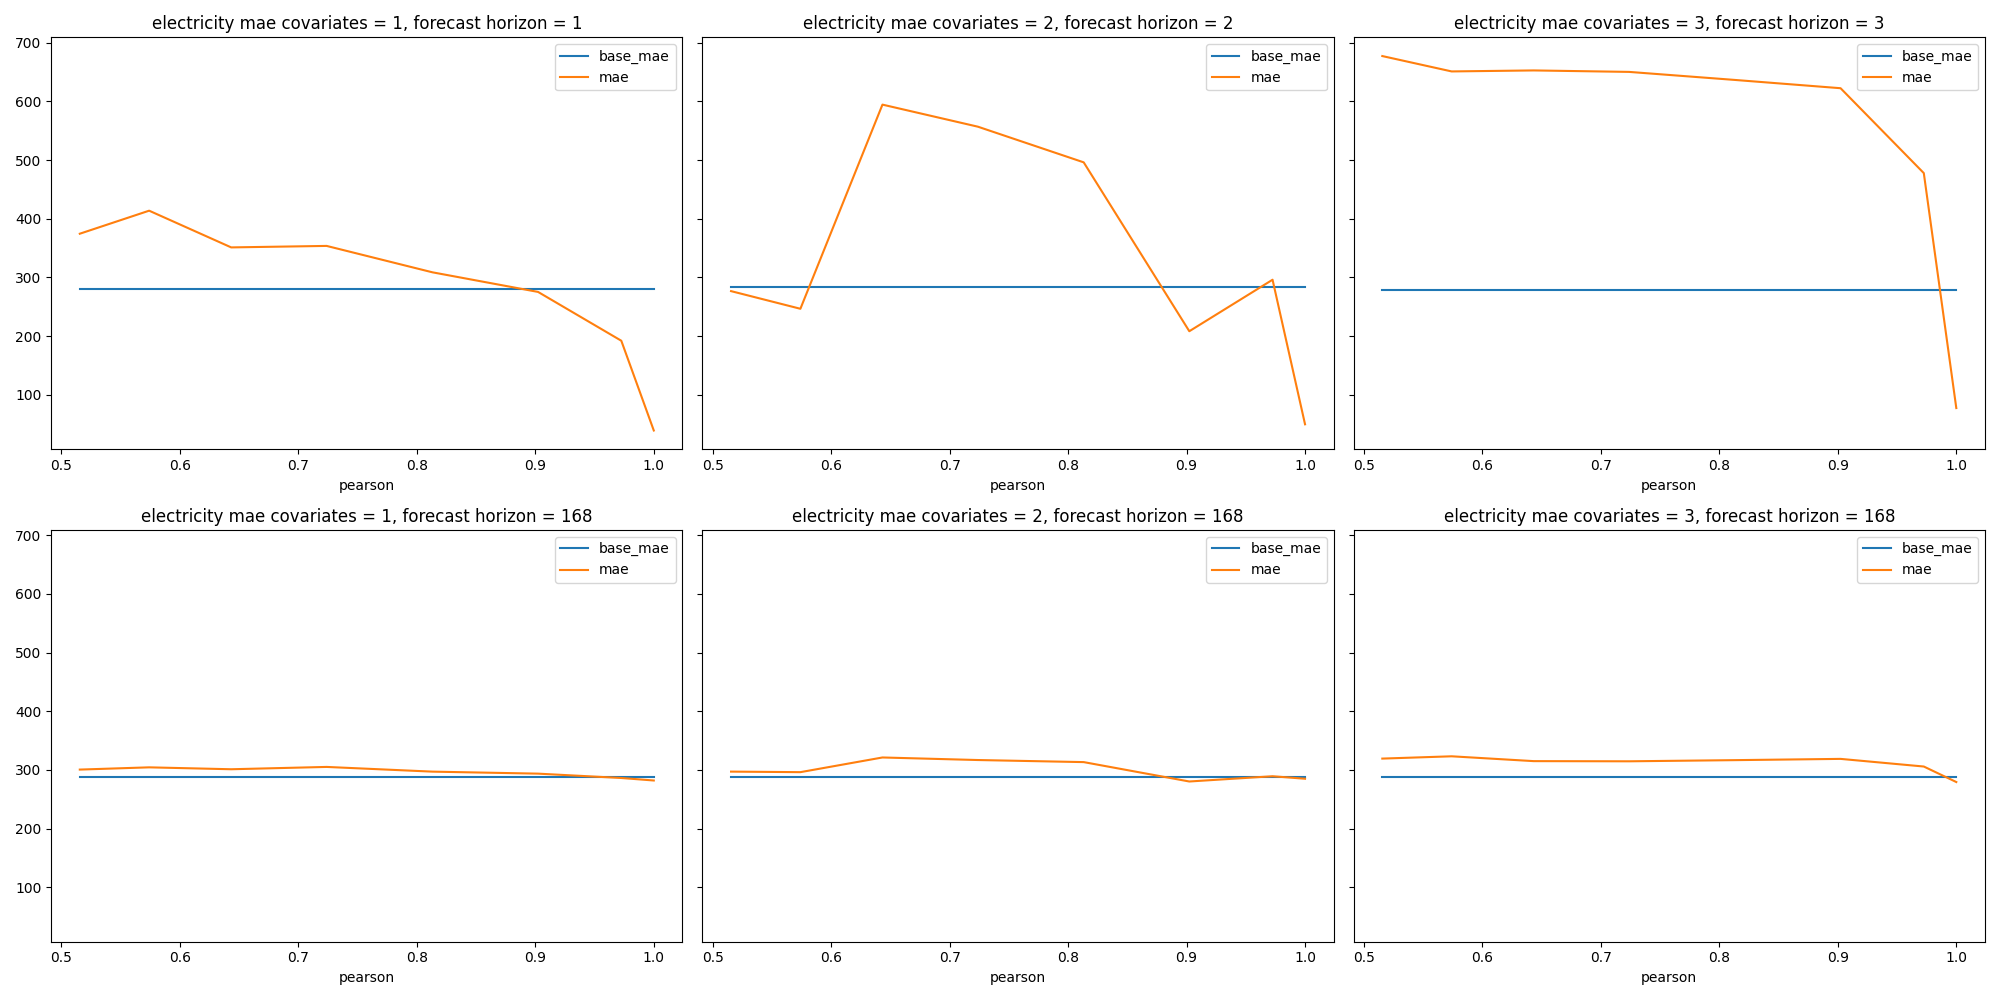
\includegraphics[width=0.9\textwidth]{figures/electricity-seg-lstm-mae.png}
  \caption{seg-lstm Electricity mae as a function of correlation for 1, 2 and 3 covariates}
  \label{fig:seg_lstm_electricity_mae}
  \end{figure}
  
  \begin{figure}[ht]
  \centering
  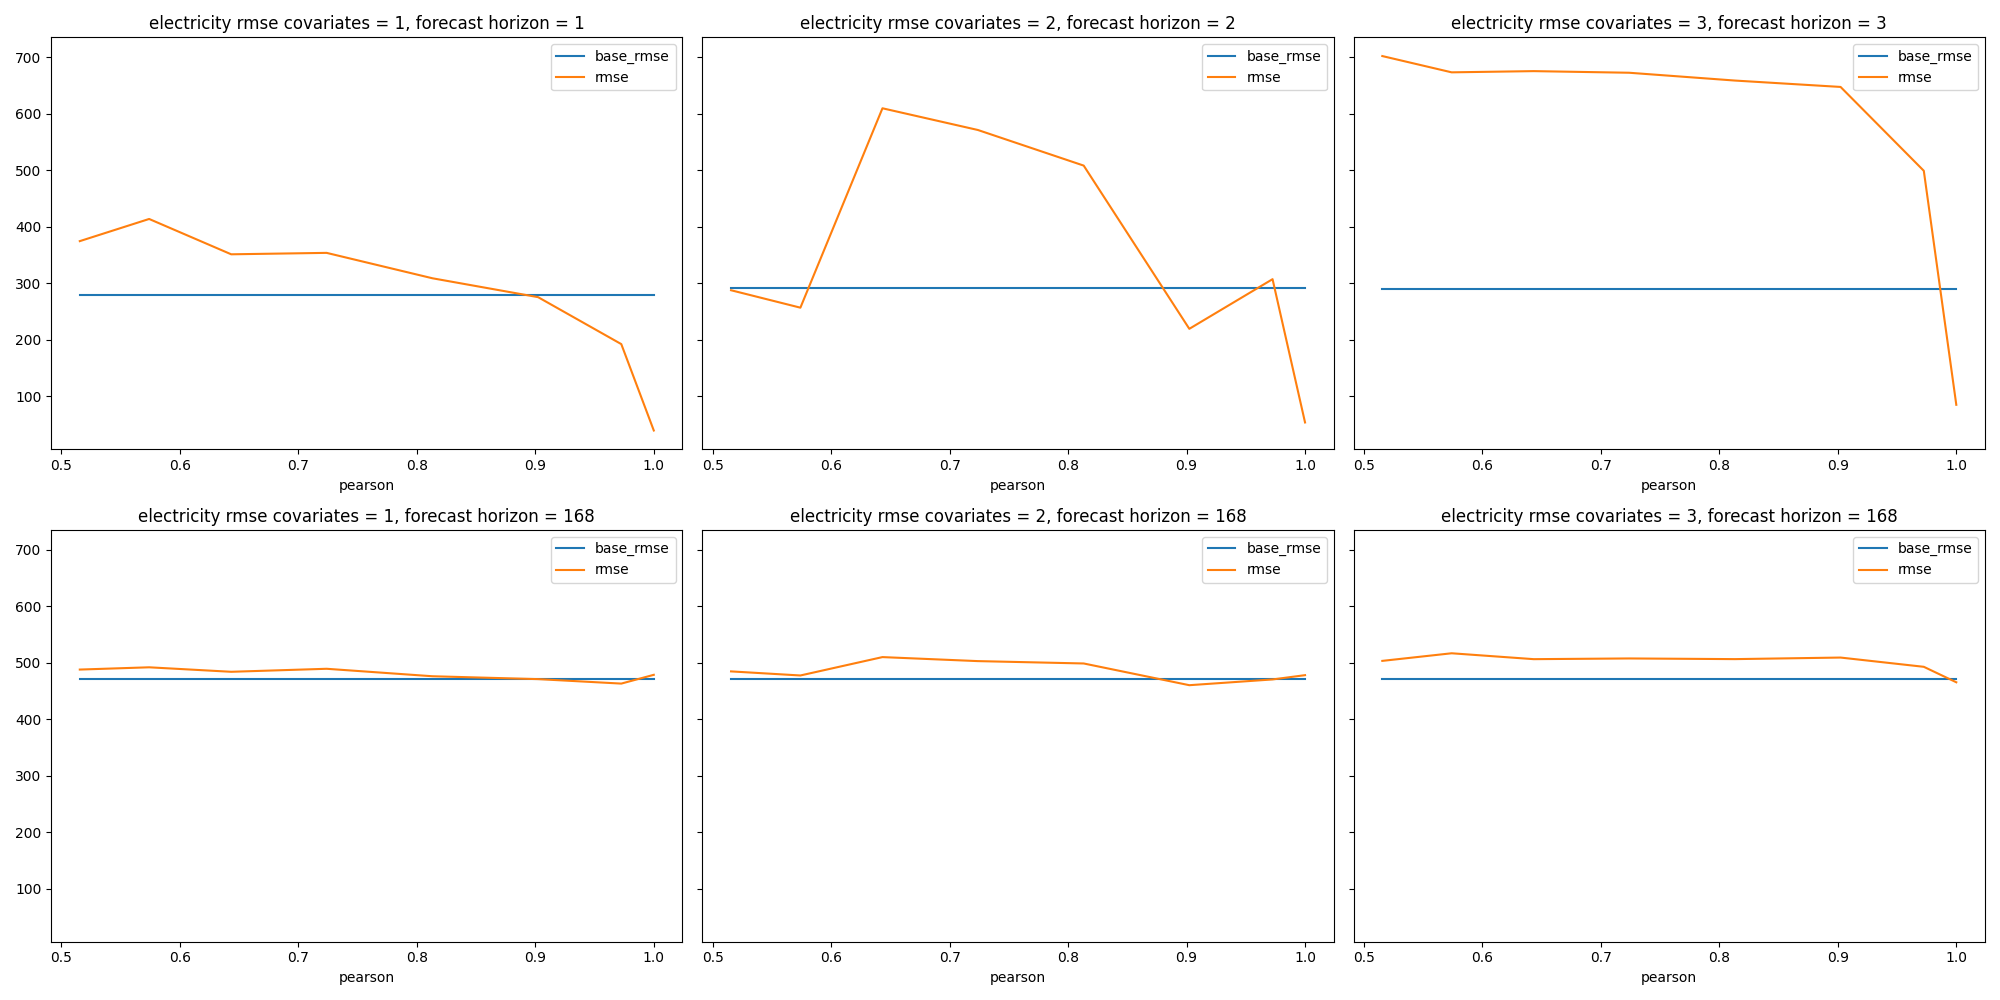
\includegraphics[width=0.9\textwidth]{figures/electricity-seg-lstm-rmse.png}
  \caption{seg-lstm Electricity rmse as a function of correlation for 1, 2 and 3 covariates}
  \label{fig:seg_lstm_electricity_rmse}
  \end{figure}

  \begin{table}[tbp]
    \caption{Multivariate results with different prediction lengths $O \in \{96,192,336,720\}$. We set the input length $I$ as 36 for ILI and 96 for the others. A lower MSE or MAE indicates a better prediction.}\label{tab:Results}
    \centering
    \begin{threeparttable}
    \begin{small}
    \renewcommand{\multirowsetup}{\centering}
    \setlength{\tabcolsep}{2.6pt}
    \begin{tabular}{c|c|cccccccccccccc}
      \toprule
      \multicolumn{2}{c}{Models} & \multicolumn{2}{c}{\textbf{Autoformer}} &  \multicolumn{2}{c}{Informer} & \multicolumn{2}{c}{LogTrans}  & \multicolumn{2}{c}{Reformer} & \multicolumn{2}{c}{LSTNet} & \multicolumn{2}{c}{LSTM} & \multicolumn{2}{c}{TCN}  \\
      \cmidrule(lr){3-4} \cmidrule(lr){5-6}\cmidrule(lr){7-8} \cmidrule(lr){9-10}\cmidrule(lr){11-12}\cmidrule(lr){13-14}\cmidrule(lr){15-16}
      \multicolumn{2}{c}{Metric} & MSE & MAE & MSE & MAE & MSE & MAE & MSE & MAE & MSE & MAE & MSE & MAE & MSE & MAE  \\
      \toprule
      \multirow{4}{*}{\rotatebox{90}{ETT$^\ast$}} & 96 & \textbf{0.255} & \textbf{0.339} & 0.365 & 0.453 & 0.768 & 0.642 & 0.658 & 0.619 & 3.142 & 1.365 & 2.041 & 1.073 & 3.041 & 1.330  \\
      & 192 & \textbf{0.281} & \textbf{0.340} & 0.533 & 0.563 & 0.989 & 0.757 & 1.078 & 0.827 & 3.154 & 1.369 & 2.249 & 1.112 & 3.072 & 1.339  \\
      & 336 & \textbf{0.339} & \textbf{0.372} & 1.363 & 0.887 & 1.334 & 0.872 & 1.549 & 0.972 & 3.160 & 1.369 & 2.568 & 1.238 & 3.105 & 1.348  \\
      & 720 & \textbf{0.422} & \textbf{0.419} & 3.379 & 1.388 & 3.048 & 1.328 & 2.631 & 1.242 & 3.171 & 1.368 & 2.720 & 1.287 & 3.135 & 1.354  \\
      \midrule
      \multirow{4}{*}{\rotatebox{90}{Electricity}} & 96  & \textbf{0.201} & \textbf{0.317} & 0.274 & 0.368 & 0.258 & 0.357 & 0.312 & 0.402 & 0.680 & 0.645 & 0.375 & 0.437 & 0.985 & 0.813  \\
      & 192  & \textbf{0.222} & \textbf{0.334} & 0.296 & 0.386 & 0.266 & 0.368 & 0.348 & 0.433 & 0.725 & 0.676 & 0.442 & 0.473 & 0.996 & 0.821  \\
      & 336  & \textbf{0.231} & \textbf{0.338} & 0.300 & 0.394 & 0.280 & 0.380 & 0.350 & 0.433 & 0.828 & 0.727 & 0.439 & 0.473 & 1.000 & 0.824  \\
      & 720  & \textbf{0.254} & \textbf{0.361} & 0.373 & 0.439 & 0.283 & 0.376 & 0.340 & 0.420 & 0.957 & 0.811 & 0.980 & 0.814 & 1.438 & 0.784  \\
      \midrule
      \multirow{4}{*}{\rotatebox{90}{Exchange}} & 96 & \textbf{0.197} & \textbf{0.323} & 0.847 & 0.752 & 0.968 & 0.812 & 1.065 & 0.829 & 1.551 & 1.058 & 1.453 & 1.049 & 3.004 & 1.432  \\
      & 192 & \textbf{0.300} & \textbf{0.369} & 1.204 & 0.895 & 1.040 & 0.851 & 1.188 & 0.906 & 1.477 & 1.028 & 1.846 & 1.179 & 3.048 & 1.444  \\
      & 336 & \textbf{0.509} & \textbf{0.524} & 1.672 & 1.036 & 1.659 & 1.081 & 1.357 & 0.976 & 1.507 & 1.031 & 2.136 & 1.231 & 3.113 & 1.459  \\
      & 720 & \textbf{1.447} & \textbf{0.941} & 2.478 & 1.310 & 1.941 & 1.127 & 1.510 & 1.016 & 2.285 & 1.243 & 2.984 & 1.427 & 3.150 & 1.458  \\
      \midrule
      \multirow{4}{*}{\rotatebox{90}{Traffic}}  & 96 & \textbf{0.613} & \textbf{0.388} & 0.719 & 0.391 & 0.684 & 0.384 & 0.732 & 0.423 & 1.107 & 0.685 & 0.843 & 0.453 & 1.438 & 0.784  \\
      & 192 & \textbf{0.616} & \textbf{0.382} & 0.696 & 0.379 & 0.685 & 0.390 & 0.733 & 0.420 & 1.157 & 0.706 & 0.847 & 0.453 & 1.463 & 0.794  \\
      & 336 & \textbf{0.622} & \textbf{0.337} & 0.777 & 0.420 & 0.733 & 0.408 & 0.742 & 0.420 & 1.216 & 0.730 & 0.853 & 0.455 & 1.479 & 0.799  \\
      & 720 & \textbf{0.660} & \textbf{0.408} & 0.864 & 0.472 & 0.717 & 0.396 & 0.755 & 0.423 & 1.481 & 0.805 & 1.500 & 0.805 & 1.499 & 0.804  \\
      \midrule
      \multirow{4}{*}{\rotatebox{90}{Weather}}  & 96 & \textbf{0.266} & \textbf{0.336} & 0.300 & 0.384 & 0.458 & 0.490 & 0.689 & 0.596 & 0.594 & 0.587 & 0.369 & 0.406 & 0.615 & 0.589  \\
      & 192 & \textbf{0.307} & \textbf{0.367} & 0.598 & 0.544 & 0.658 & 0.589 & 0.752 & 0.638 & 0.560 & 0.565 & 0.416 & 0.435 & 0.629 & 0.600  \\
      & 336 & \textbf{0.359} & \textbf{0.395} & 0.578 & 0.523 & 0.797 & 0.652 & 0.639 & 0.596 & 0.597 & 0.587 & 0.455 & 0.454 & 0.639 & 0.608  \\
      & 720 & \textbf{0.419} & \textbf{0.428} & 1.059 & 0.741 & 0.869 & 0.675 & 1.130 & 0.792 & 0.618 & 0.599 & 0.535 & 0.520 & 0.639 & 0.610  \\
      \midrule
      \multirow{4}{*}{\rotatebox{90}{ILI}}  & 24   & \textbf{3.483} & \textbf{1.287} & 5.764 & 1.677 & 4.480 & 1.444 & 4.400 & 1.382 & 6.026 & 1.770 & 5.914 & 1.734 & 6.624 & 1.830  \\
      & 36   & \textbf{3.103} & \textbf{1.148} & 4.755 & 1.467 & 4.799 & 1.467 & 4.783 & 1.448 & 5.340 & 1.668 & 6.631 & 1.845 & 6.858 & 1.879  \\
      & 48   & \textbf{2.669} & \textbf{1.085} & 4.763 & 1.469 & 4.800 & 1.468 & 4.832 & 1.465 & 6.080 & 1.787 & 6.736 & 1.857 & 6.968 & 1.892  \\
      & 60   & \textbf{2.770} & \textbf{1.125} & 5.264 & 1.564 & 5.278 & 1.560 & 4.882 & 1.483 & 5.548 & 1.720 & 6.870 & 1.879 & 7.127 & 1.918  \\
      \bottomrule
    \end{tabular}
    
    \end{small}
     \begin{tablenotes}
          \footnotesize
          \item[*] \emph{ETT} means the ETTm2. See Appendix  for the \textbf{full benchmark} of ETTh1, ETTh2, ETTm1.
    \end{tablenotes}
    \end{threeparttable}
    \vspace{-15pt}
  \end{table}



  smape	covariates	base-lstm			seg-lstm		
		1	0.9	0.5	1	0.9	0.5
Hospital	0				18.05 ± 0.135	18.05 ± 0.135	18.05 ± 0.135
	1				16.47	18.06	18.39
	2				14.87	18.09	18.12
	3				13.96	18.24	18.62

\subsection{hyperparameters}
\begin{table}[htbp]
  \centering
  \begin{tblr}{
    vline{-} = {1-11}{},
    hline{1-12} = {-}{},
  }
  learning rate           & 0.001    \\
  epochs                  & 100      \\
  hidden cells            & 40       \\
  lstm hidden layers      & 2        \\
  dropout                 & 0.1      \\
  weight decay            & 1e-8     \\
  batch size              & 128      \\
  batches per epoch       & 200      \\
  early stopping patience & 30       \\
  optimizer               & AdamW    \\
  scheduler               & OneCycle \\
                          &          
  \end{tblr}
\caption{Hyperparameters}
\label{hyperparameters}
  \end{table}

%%%%%%%%%%%%%%%%%%%%%%%%%%%%%%%%%%%%%%%%%%%%%%%%%%%%%%%%%%%%

\end{document}